\documentclass[11pt]{article}

\usepackage[margin=1in]{geometry}
\usepackage{amsmath,amssymb,amsthm,mathtools}
\usepackage{booktabs}
\usepackage{graphicx}
\usepackage{microtype}
\usepackage{natbib}
\usepackage[hidelinks]{hyperref}
\usepackage[nameinlink,noabbrev]{cleveref}

\newtheorem{theorem}{Theorem}[section]
\newtheorem{proposition}[theorem]{Proposition}
\newtheorem{lemma}[theorem]{Lemma}
\newtheorem{corollary}[theorem]{Corollary}
\newtheorem{conjecture}[theorem]{Conjecture}
\theoremstyle{definition}
\newtheorem{definition}[theorem]{Definition}
\theoremstyle{remark}
\newtheorem{remark}[theorem]{Remark}

\newcommand{\R}{\mathbb{R}}
\newcommand{\E}{\mathbb{E}}
\newcommand{\cL}{\mathcal{L}}
\newcommand{\norm}[1]{\left\lVert #1\right\rVert}
\newcommand{\od}{\mathbin{\odot}}
\newcommand{\dd}{\,\mathrm{d}}
\newcommand{\diag}{\operatorname{diag}}
\newcommand{\Law}{\operatorname{Law}}
\newcommand{\HS}{\mathrm{HS}}

\title{{\fontsize{14}{17}\selectfont\bfseries
Compressing Global Dynamics of Deep Nonlinear Feature Learning}}
\author{Amir Joudaki}
\date{September 27, 2026}

\begin{document}
\maketitle

\begin{abstract}
How much can the training dynamics of a deep network be compressed?  A snapshot
of a trained network is easy to compress; its training is not, because networks
that agree on every input can drift apart once training resumes.  We ask how
small a state suffices to reproduce the \emph{whole} training trajectory while
keeping depth, effective nonlinearity and feature learning, because the state
that survives is a candidate for the variables that govern learning.  Existing
exact descriptions of feature learning compress \emph{width} but not
\emph{time}: Tensor Programs and dynamical mean-field theory keep the full history
of forward and backward responses, and we collect evidence that exact capture is
possible only through operator equations that carry the whole learned matrix.
We show that the history itself is compressible.  Measured in a clock that runs
at the speed of learning, each neuron's forward and backward response history is
summarized by $P$ shifted-Legendre moments.  The resulting autonomous system has
a state that does not grow with training time and, for networks of any depth,
tracks the whole parameter trajectory with error $O_T(P^{-1})$, or $O_T(P^{-2})$
with a second, joint clock.  The mechanism is that pairing forward and backward
memories makes the error in each weight update a product of two projection
errors.  As a corollary, on any finite horizon every learned weight increment
lies within $O(1/P)$ of a rank-$mP$ matrix built from the network's own response
moments.  On circle and MNIST tasks, orders $P=2$--$3$ reproduce the dense
predictor over the whole input space, while frozen or directly trained low-rank
bases of the same size do not.  Placed on a common axis of evolving state
against accuracy, existing descriptions of training pay for the limit in
neurons, in stored history or in tuples of samples; response memory pays in an
approximation order.
\end{abstract}

\section{Introduction}

\paragraph{A missing model of learning.}
The Turing machine is the canonical model of computation.  It is idealized---it
has no limit on memory or precision---and it is simple enough to reason about,
while physical computers, from the von Neumann architecture onward, are
understood as its finite-resource implementations.  One may argue that the Turing
machine is a model of computing rather than of learning, and that learning still
lacks its canonical idealized model.  Deep neural networks trained by gradient
descent are the obvious candidates for implementations of such a model, but the
object they would implement is not yet known.  The obstacle is that their
training dynamics are enormously complex and have no simple representation.

\paragraph{Why look in the limit.}
A natural place to look for the idealized object is the limit of infinite width.
Under feature-learning scalings of the type used in tensor-program and mean-field
theory \citep{yang2021tensor,nguyen2023rigorous}, width and learning rate are
absorbed into the parametrization and the quantities we care about---predictions,
kernels, the laws of hidden neurons---evolve deterministically.  The limit is the
network with no resource constraint, as the Turing machine is the computer with
none.  A finite network would then be understood as this limit plus a quantified
deviation from it, a CLT-style picture in which each finite network combines its
idealized limit with fluctuations around it.

\paragraph{Why compression.}
Going to infinite width to simplify seems paradoxical: the dynamical system grows
with width and becomes infinite in the limit.  Statistical physics resolves the
paradox in other settings.  A gas of $10^{23}$ molecules is simpler to describe
than a gas of ten, because its macroscopic behaviour is captured by a few
collective variables; mean-field theory replaces intricate particle interactions
by smooth population fields.  For training, however, the limit is infinite in
two directions: in the number of neurons, and in time, because the state of
training depends on the whole history of how each neuron has responded.
Mean-field and tensor-program limits tame the first.  Whether the second can be
tamed as well is the question of whether the limiting training dynamics can be
\emph{compressed}.  We do not seek compression for its own sake.  A compressed
description must retain what drives learning and may discard the rest, so the
state that survives is a candidate for the variables that govern learning, and
a compressed system that reproduces training would be a step toward the
idealized model.

\paragraph{Training, not snapshots.}
Compressing a snapshot is easy: any representation of the current input--output
map will do.  But two networks that compute the same function on every input can
have different Jacobians and backward responses, and once training resumes the
discrepancy accumulates.  An idealized model of learning must reproduce the whole
trajectory.

\paragraph{What the model must keep.}
Several idealized models of training already exist, and each gives up one of
three properties.  Deep linear networks admit exact solutions but lose the
nonlinearity \citep{saxe2014exact}; mean-field analyses are largely confined to
one hidden layer \citep{chizat2018global,mei2018meanfield,sirignano2019lln}; and
the neural tangent kernel keeps depth and nonlinearity but freezes the features
\citep{jacot2018ntk,lee2019wide,chizat2019lazy}.  Each is simple precisely
because of what it gives up.  We keep all three: \emph{depth} (more than one
hidden layer), \emph{nonlinearity} that stays effective during training and in
the limit, and \emph{feature learning} (hidden representations move at leading
order).  Together with the population limit, this contract preserves what is
hardest about deep learning while making it a single well-defined object.

\paragraph{The gap.}
Existing exact descriptions of this object do not compress it.  Tensor Programs
carry variables indexed by every earlier training step \citep{yang2021tensor},
and feature-learning dynamical mean-field theory (DMFT) evolves two-time kernels
whose memory grows quadratically with the number of time points
\citep{bordelon2022dmft}.  Both are remarkable statements about the network's
behaviour, and both are exact; but they avoid storing the learned matrix only by
storing the history of forward and backward responses from which it is built.
The information is moved rather than compressed.  In the terms above, these
descriptions tame the infinity in \emph{width}---their state does not depend on
the number of neurons---but not the one in \emph{time}: their state grows with
the length of training.
No result we know of shows that deep nonlinear feature learning can be captured
by a system whose size stays constant throughout training.

\paragraph{One axis for every description.}
The gap suggests a way to place all descriptions of training side by side.  Fix
a horizon and an accuracy, and ask how much \emph{evolving} state a description
needs to reproduce the trajectory to that accuracy, and whether that state grows
with the length of training.  Descriptions that freeze the features, drop depth
or drop the nonlinearity are not approximations of the object in our contract at
any size: enlarging their state does not bring them closer to it, so they sit
off this axis, exact about something else.  The descriptions that keep the
contract sit on it, and each pays for the limit in a different currency: the
dense network in neurons, Tensor Programs and DMFT in stored history, the Neural
Tangent Hierarchy in tensors indexed by tuples of training samples.  Response
memory pays in an approximation order, which depends neither on the length of
training nor on the combinatorics of the samples.  \Cref{sec:notions} makes the
axis precise, \Cref{tab:axis} places the descriptions on it, and \Cref{app:size}
works out, under stated hypotheses, what each would cost at a prescribed
accuracy.

\paragraph{Results.}
\Cref{sec:notions} makes compression of dynamics precise and distinguishes three
classes of state: scalars, populations and operators.  We then show the
following.
\begin{enumerate}
\item \emph{Exact capture points to operators} (\Cref{sec:exact}).  Three pieces
of evidence---an exact operator closure for deep linear networks, an exact but
never-closing hierarchy of current observations for a two-hidden-layer network,
and a restricted failure of scalar closures---suggest that
exact capture of deep nonlinear feature learning requires operator equations,
which compress nothing.  We do not prove this.
\item \emph{Training history is compressible in time} (\Cref{sec:memory}).  For
networks of any depth, replacing each neuron's forward and backward history by
$P$ Legendre moments in a learning-speed clock gives an autonomous system whose
state does not grow with training time and whose trajectory is within
$O_T(P^{-1})$ of gradient flow, or $O_T(P^{-2})$ with a joint clock
(\Cref{thm:old,thm:new}).  The difficulty is feedback: the memorized signals
depend on the approximation itself.
\item \emph{A structural consequence} (\Cref{cor:rank}).  Every learned weight
increment is, on a finite horizon, within $O(1/P)$ of a rank-$mP$ matrix built
from the network's own response moments.
\item \emph{Evolving memories are what matter} (\Cref{sec:experiments}).  Small
orders reproduce the dense predictor over the whole input space, while, in our
comparisons, frozen dictionaries and directly trained low-rank corrections of
the same size fail.
\end{enumerate}
The theorems hold at every fixed width.  The population limit is the motivation
and gives an interpretation of the result (\Cref{sec:population-view}), and a
precise conjecture (\Cref{conj:population}) states what a population version
would be; it is not proved here.  \Cref{app:popclosure} records an earlier,
weaker closure of the population flow itself, in which the learned middle layer
is confined to a frozen span of initialization observables; it converges without
a rate, and its limitations motivated the evolving memories of the main result.

\section{Related work}
\label{sec:related}

We organize prior work by where it sits on the axis of the introduction: whether
it approximates the deep nonlinear feature-learning flow at all, and, if it
does, in what currency its evolving state is paid.

\paragraph{Off the axis: descriptions that give up one property.}
Exact solutions of deep linear networks keep depth and feature learning but not
nonlinearity \citep{saxe2014exact}; their infinite-width limit is a gradient
flow on $\ell^2$ operators added to the frozen initialization
\citep{chizat2024linear}, the cleanest example of an operator description.
Wasserstein and mean-field limits describe one-hidden-layer networks as the
gradient flow of a measure over neurons
\citep{chizat2018global,mei2018meanfield,sirignano2019lln}; they keep nonlinear
feature learning but not depth.  The neural tangent kernel and lazy training
keep depth and nonlinearity but freeze the features, reducing training to a
fixed kernel \citep{jacot2018ntk,lee2019wide,chizat2019lazy}.  Each is simple
because of what it sacrifices, and each is exact about a different object.
None is an approximation of ours whose error can be driven down by enlarging
its state; for the frozen kernel in particular, the discrepancy from a
feature-learning flow is a bias that width does not remove.

\paragraph{On the axis, paying in history.}
Tensor Programs~IV proves feature-learning limits at each fixed number of steps,
with a recursion that includes variables indexed by every earlier step
\citep{yang2021tensor}.  Feature-learning DMFT evolves two-time activation,
gradient and response kernels, with memory quadratic and time cubic in the
number of time points \citep{bordelon2022dmft}, and its finite-width extension
adds perturbative fluctuations \citep{bordelon2023finite}.  Its own comparison
is that DMFT is cheaper than the network only when $n\gg mK$, $K$ the number of
grid points; a numerical solution further needs Monte Carlo samples of the
single-site processes and self-consistency sweeps, which that count leaves out.
Multilayer mean-field theory and Neural Feature Flow evolve fields on neuronal
ensembles \citep{nguyen2023rigorous,fang2020features}.  These keep all three
properties and identify the idealized object.  They compress width: DMFT, for
instance, has a state independent of the number of neurons.  But their state
grows with the length of training, or consists of infinite-dimensional fields.
Our result is complementary: it keeps the neurons and compresses time.

\paragraph{On the axis, paying in tuples of samples.}
The Neural Tangent Hierarchy \citep{huang2020nth} evolves the outputs together
with the tangent kernels of order $2,\dots,p$, the $r$-th a function of $r$
training points, and closes by freezing the top kernel.  The hierarchy is an
exact identity in any parametrization, and above order two it captures feature
learning; the neural tangent kernel is its lowest truncation.  What it pays is
combinatorial in the samples: the moving state through order $p$ is
$\sum_{r<p}m^r$ scalars beneath a frozen tensor of $m^p$ entries (a direct
count rather than a statement of that work), against a state linear in $m$
here.  Its guarantee is proved in the parametrization where each kernel is
smaller than the previous by $n^{-1/2}$, so that truncation costs $n^{-p/2}$:
the error decreases in width, grows polynomially in time, and holds on a
width-dependent horizon.  It is an expansion around the lazy limit in the small
parameter $t/\sqrt n$.  In the feature-learning parametrization the kernels move
at order one, and the truncation error is governed instead by the growth of the
higher kernels, for which no general bound is available (\Cref{app:size}).
Response memory controls the full parameter trajectory at fixed width, with a
state linear in $P$ and an error decreasing polynomially in $P$.

\paragraph{Memory and low rank.}
HiPPO provides online Legendre projection of a given signal \citep{gu2020hippo};
we apply it to endogenous, coupled training histories and prove stability of the
resulting feedback loop.  Low-rank training methods constrain the learned
increment to evolving factors \citep{zhao2023inrank}; response-memory factors are
causal summaries of the actual forward and backward histories, and a directly
trained factorization of matched rank performs far worse
(\Cref{sec:experiments}).

\section{Setting}
\label{sec:setting}

Fix $m$ training pairs $(x_a,y_a)$ with $x_a\in\R^d$, width $n$ and $H\ge2$
hidden layers:
\begin{align}
 z_a^{(1)}&=W^{(1)}x_a/\sqrt d,& h_a^{(1)}&=\phi(z_a^{(1)}),\nonumber\\
 z_a^{(\ell)}&=W^{(\ell)}h_a^{(\ell-1)},&
 h_a^{(\ell)}&=\phi(z_a^{(\ell)}),\quad 2\le\ell\le H,\\
 f_a&=\frac{w^\top h_a^{(H)}}{n},& r_a&=f_a-y_a,\qquad
 \rho=\Bigl(\frac1m\sum_a r_a^2\Bigr)^{1/2}.\nonumber
\end{align}
The activation $\phi$ may differ between layers; the loss is $\cL=\rho^2$.  The
backward responses, which exclude the residual, are
$\delta_a^{(H)}=w\od\phi'(z_a^{(H)})$ and
$\delta_a^{(\ell)}=\phi'(z_a^{(\ell)})\od(W^{(\ell+1)})^\top\delta_a^{(\ell+1)}$.
With block mobilities $(n,1,\ldots,1,n)$, gradient flow reads
\begin{equation}
 \dot W^{(1)}=-\frac2m\sum_a r_a\delta_a^{(1)}\frac{x_a^\top}{\sqrt d},\quad
 \dot W^{(\ell)}=-\frac{2}{nm}\sum_a r_a\delta_a^{(\ell)}
 (h_a^{(\ell-1)})^\top\ (2\le\ell\le H),\quad
 \dot w=-\frac2m\sum_a r_a h_a^{(H)}.\label{eq:dense-flow}
\end{equation}
We write $\theta=(W^{(1)},\ldots,W^{(H)},w)$ for all parameters and
$\dot\theta=F(\theta)$ for \eqref{eq:dense-flow}.  Hidden entries are initialized
as $\mathcal N(0,1/n)$, first-layer entries as $\mathcal N(0,1)$, and the stored
readout is small.

\paragraph{Population flow.}
As $n\to\infty$, the neurons of layer $\ell$ become a probability space
$\Omega_\ell$ with expectation $\E_\ell$: hidden coordinates $z^{(\ell)},h^{(\ell)}$
become random variables in $L^2(\Omega_\ell)$, the first-layer weights a random
row $W^{(1)}\in L^2(\Omega_1;\R^d)$, the readout $w\in L^2(\Omega_H)$, and each
hidden matrix a bounded operator $W^{(\ell)}:L^2(\Omega_{\ell-1})\to L^2(\Omega_\ell)$
used together with its true adjoint.  The same equations \eqref{eq:dense-flow}
hold with $\frac1n\sum_i$ replaced by $\E_\ell$ and outer products
$\delta\,h^\top/n$ by the rank-one operators $g\mapsto\delta\,\E[h\,g]$.  Such
limits are established in several scopes---for fixed depth on a short horizon,
and globally in special models---with finite-width gradient flow converging to
them on compact horizons; a global theorem for general data and depth is open.
Where we need the population flow we state its existence as part of the model.

\section{Compressing a dynamical system}
\label{sec:notions}

\paragraph{Exact and approximate; local and global.}
An exact compression reproduces the reference trajectory; an approximate one
reproduces it up to a controllable error.  A compression may also match the
current state and velocity while its small errors compound until the
trajectories separate; we ask for the stronger, global notion.

\begin{definition}[Global approximation on compact horizons]
\label{def:global}
Autonomous systems indexed by an order $N$, with trajectories $\theta_N$,
\emph{globally approximate} a reference flow $\theta$ if for every $T<\infty$
\[
  \sup_{0\le t\le T}\norm{\theta_N(t)-\theta(t)}\longrightarrow0
  \qquad(N\to\infty).
\]
The rate in $N$ quantifies the trade-off between the size of the compressed
state and its accuracy.
\end{definition}

\paragraph{Size against accuracy.}
\Cref{def:global} compares one compression with its reference.  To compare
different descriptions of training with each other we fix the reference and ask
what each costs.  Call the \emph{moving state} of a description the numbers it
updates while computing training, excluding fixed sources such as the
initialization or a frozen kernel.

\begin{definition}[Size at accuracy]
\label{def:size}
For a description of training, a horizon $T$ and an accuracy $\varepsilon$, let
$M(\varepsilon;T)$ be the smallest moving state with which it reproduces the
reference trajectory on $[0,T]$ to within $\varepsilon$.  The description
\emph{compresses time} if $M(\varepsilon;T)$ depends on $T$ only through the
constants of its error bound and not through a count of elapsed steps.
\end{definition}

A description that does not approximate the reference has
$M(\varepsilon;T)=\infty$ below some $\varepsilon$; this is how the three
properties of the contract act, since dropping any one of them leaves a bias
that no state removes.  \Cref{tab:axis} places the descriptions of
\Cref{sec:related} on this axis by what their moving state is indexed by, what
grows, and against what their error is certified.  The entries are orders of
magnitude, not a ranking: constants differ between rows, and several rows
depend on hypotheses named in the last column.  \Cref{sec:size} states what the
theorems of this paper give at fixed width, and \Cref{app:size} works out the
conditional population-level version.

\begin{table}[t]
\centering
\footnotesize
\setlength{\tabcolsep}{4pt}
\caption{Descriptions of the same training flow on one axis.  $m$ samples,
$n$ width, $H$ hidden layers, $K$ time steps, $p$ kernel order, $P$ moment
order.  Moving state excludes fixed sources; the frozen
$W_0$ ($Hn^2$), NTH's top tensor ($m^p$) and the NTK matrix ($m^2$) are fixed.
``Certified against'' names the reference for which an error bound exists;
(H1), (H3) are the hypotheses of \Cref{app:size}.}
\label{tab:axis}
\begin{tabular}{@{}llllll@{}}
\toprule
Description & Gives up & Indexed by & Moving state & Grows? & Certified against\\
\midrule
\multicolumn{6}{@{}l}{\emph{Off the axis: exact about a different object}}\\
Deep linear & nonlinearity & modes & --- & no & its own limit\\
Shallow mean field & depth & particles & $n$ & no & its own limit\\
Neural tangent kernel & features & samples & $m$ & no & lazy limit only\\
\midrule
\multicolumn{6}{@{}l}{\emph{On the axis: pays for the limit in a currency}}\\
Dense network & --- & neurons & $Hn^2$ & no & population, (H1)\\
Stored history & --- & past steps & $HmnK$ & $\propto K$ & finite net, exact\\
Tensor Programs & --- & past steps & grows & yes & population, no rate\\
DMFT solver & --- & sample, time pairs & $Hm^2K^2$ & $\propto K^2$ & population, (H3)\\
NTH, order $p$ & --- & sample tuples & $\sum_{r<p}m^r$ & no & finite net, lazy param.\\
Response memory, speed clock & --- & neuron moments & $2HmnP$ & no & finite net, $P^{-1}$\\
Response memory, joint clock & --- & neuron moments & $2HmnP+P^2$ & no & finite net, $P^{-2}$\\
\bottomrule
\end{tabular}
\end{table}

\paragraph{Three classes of state.}
\begin{enumerate}
\item A \emph{scalar ODE} evolves finitely many real numbers, independently of
width and training time.
\item A \emph{population} (or field) ODE evolves finitely many functions, random
variables or probability laws on fixed spaces---for example the law of a neuron's
weights.  Its particle implementation stores one value per particle and field;
the number of objects is finite, their degrees of freedom are not.
\item An \emph{operator} ODE evolves operators between population spaces, the
limits of matrices.  A matrix records how \emph{each} row relates to \emph{each}
column, and this row--column coupling cannot in general be captured by finitely
many populations.
\end{enumerate}
A finite number of named fields or operators need not contain finitely many
scalars, so every compression claim below names both the type and the size of
the retained state.

\section{Exact compression: evidence that it lives in the operator class}
\label{sec:exact}

Before allowing errors we ask what exact capture of the population flow can look
like.  We do not settle this question; we collect three pieces of evidence that
point the same way.

\paragraph{An exact operator description exists, and is finite only in name.}
If we refuse the growing histories of Tensor Programs and DMFT, the natural
exact description of the population flow is an operator ODE: \eqref{eq:dense-flow}
read with the hidden matrices $W^{(\ell)}$ as operators.  In a deep linear
benchmark---one input, three linear hidden layers, order-one initialization---this
can be proved completely: the learned part of the whole network becomes a single
trace-class operator that evolves by an explicit autonomous cubic equation
driven by the residual, and finite gradient flow and gradient descent converge
to it on every compact horizon (\Cref{app:exact}).  The description is exact and
consists of one operator, but that operator is as rich as the learned matrix:
any finite approximation of it essentially stores either the dense matrix or the
responses that built it.

\paragraph{The past can be dropped, but only for an infinite hierarchy.}
For a two-hidden-layer population flow on the circle (\Cref{app:popclosure}), one can
describe the dynamics exactly through \emph{current} observations: joint laws,
on each neuron population, of finitely many expressions built from the current
weights, the initialization, $\phi$, bounded products and applications of
$W^{(2)}$ and its adjoint.  The derivative of each finite level of this
hierarchy is expressed through a finite higher level, and the complete hierarchy
determines predictions on the whole input space and a unique continuation from
every reachable state, without storing the past.  But no finite level closes.

\paragraph{Exact scalar closures fail.}
In the same linear benchmark, no encoder formed from a fixed finite list of
tensor contractions of the weights with width-independent bounded degree admits
a polynomial autonomous scalar ODE and polynomial readout that reproduce the
output dynamics on an open set of states at all large widths (\Cref{app:exact}).
The reason is that repeated differentiation of the output forces ever larger
connected contractions: the $(2j-1)$st derivative contains
\[
 \frac1n\,(W^{(1)})^\top\Bigl((W^{(2)})^\top(W^{(3)})^\top W^{(3)}W^{(2)}\Bigr)^{j}W^{(1)},
\]
of degree $4j+2$, which no bounded-degree alphabet can express.  The result is
restricted to a natural class of encoders, but if exact scalar closure fails for
three \emph{linear} layers, there is little reason to expect it for nonlinear
feature learning.

\paragraph{Between the two.}
Whether the exact operator can be compressed into finitely many populations is
open.  We believe not: natural reductions of an operator to populations assume
structure, such as finite rank, that feature learning does not provide, since
gradient flow integrates rank-one updates over continuous time.  Taken together,
the evidence suggests that exact capture of deep nonlinear feature learning is
possible only in the operator class, which hides a growing complexity in finite
clothing.  The rest of the paper asks what can be gained by accepting a
controlled error.

\section{Approximate compression with rates: response memories}
\label{sec:memory}

We now ask what can be gained by accepting a controlled error, for networks of
any depth and with explicit order-versus-error rates.

\subsection{The idea}

Integrating \eqref{eq:dense-flow}, every hidden matrix is
\begin{equation}
 W^{(\ell)}(t)=W_0^{(\ell)}-\frac{2}{nm}\sum_a
 \int_0^t r_a(s)\,\delta_a^{(\ell)}(s)\,
 (h_a^{(\ell-1)}(s))^\top\dd s .                        \label{eq:exact-history}
\end{equation}
The learned part is an integral of backward against forward responses.  Storing
it means storing the dense matrix or the whole response history.  But to predict
where a moving ball goes next we need its position, velocity and acceleration,
not its past positions.  If each response history is regular in time, a few
coefficients should summarize it.  Two things must hold: the summary must be
\emph{closed}, so that it evolves autonomously, and \emph{accurate} over the
whole of training, which alternates between bursts of learning and plateaus.

\subsection{Closure: shifted Legendre moments}

Let $p_k$ be the shifted Legendre polynomials on $[0,1]$, normalized by
$p_k(1)=1$ and $\int_0^1p_jp_k=\mathbf 1_{j=k}/(2k+1)$.  Their derivatives reduce
to lower modes,
\begin{equation}
 x\,p_k'(x)=k\,p_k(x)+\sum_{j<k}(2j+1)\,p_j(x),        \label{eq:triangular}
\end{equation}
and this is what makes the moment system close exactly.  The identity underlies
online polynomial memory in HiPPO \citep{gu2020hippo}; the new element is that
the memorized signals are the network's own forward and backward responses,
coupled back through the reconstructed network.

\subsection{Accuracy: a clock that follows learning}

A polynomial basis is accurate only if history is spread evenly over its window,
and in physical time it is not.  We therefore measure history in a clock
$\tau$ that runs at the speed of learning,
\begin{equation}
 \dot\tau=\rho,\qquad \tau(0)=1:                        \label{eq:old-clock}
\end{equation}
fast while the network learns, slow as learning stalls.  The unit prefix
$[0,1]$ carries the initial forward responses and no backward response.  For
each hidden link $\ell\ge2$ and sample $a$ we store the first $P$ Legendre
moments, in the clock coordinate, of the forward response $h_a^{(\ell-1)}$ and
of the residual-weighted backward response $r_a\delta_a^{(\ell)}/\rho$:
\[
 \bar h^{(\ell-1)}_{a,k}=\int_0^{\tau} h_a^{(\ell-1)}\,p_k(\xi/\tau)\dd\xi,\qquad
 \bar\delta^{(\ell)}_{a,k}=\int_0^{\tau}\frac{r_a\delta_a^{(\ell)}}{\rho}\,
 p_k(\xi/\tau)\dd\xi,\qquad 0\le k<P,
\]
where $\xi$ is the clock value at which each response was recorded.  By
\eqref{eq:triangular} these moments obey the closed system
\begin{align}
 \dot{\bar h}^{(\ell-1)}_{a,k}&=\rho\,h_a^{(\ell-1)}-\frac{\rho}{\tau}
 \Bigl[k\,\bar h^{(\ell-1)}_{a,k}+\sum_{j<k}(2j+1)\,\bar h^{(\ell-1)}_{a,j}\Bigr],\nonumber\\
 \dot{\bar\delta}^{(\ell)}_{a,k}&=r_a\delta_a^{(\ell)}-\frac{\rho}{\tau}
 \Bigl[k\,\bar\delta^{(\ell)}_{a,k}+\sum_{j<k}(2j+1)\,\bar\delta^{(\ell)}_{a,j}\Bigr],
 \label{eq:old-ode}
\end{align}
with $\bar h^{(\ell-1)}_{a,0}(0)=h_a^{(\ell-1)}(0)$ and all other moments zero, and
the hidden matrices are reconstructed as
\begin{equation}
 \widehat W^{(\ell)}=W_0^{(\ell)}-\frac{2}{nm\tau}
 \sum_{a=1}^m\sum_{k=0}^{P-1}(2k+1)\,
 \bar\delta^{(\ell)}_{a,k}\,(\bar h^{(\ell-1)}_{a,k})^\top .   \label{eq:old-recon}
\end{equation}
All responses in \eqref{eq:old-ode} are evaluated in the current
\emph{reconstructed} network, and the first layer and readout follow
\eqref{eq:dense-flow}.  The system is autonomous and never divides by $\rho$.
Equivalently, with $\Pi_P$ the $L^2(0,\tau)$ projection onto polynomials of
degree below $P$,
\begin{equation}
 \widehat W^{(\ell)}=W_0^{(\ell)}-\frac{2}{nm}\sum_a
 \int_0^\tau\Bigl(\Pi_P\frac{r_a\delta_a^{(\ell)}}{\rho}\Bigr)
 \bigl(\Pi_Ph_a^{(\ell-1)}\bigr)^\top\dd\xi,               \label{eq:projection-form}
\end{equation}
and since cross terms vanish by orthogonality, the error in each matrix update is
a \emph{product} of a forward and a backward projection error.

\paragraph{The joint feature-learning clock.}
The learning-speed clock makes forward histories smooth but not every backward
history.  A second clock advances with the residual \emph{plus} the speed of all
forward and backward responses,
\begin{equation}
 \dot\tau=\rho+\Bigl\|\tfrac{d}{dt}\bigl(h_a^{(\ell-1)},\,r_a\delta_a^{(\ell)}/\rho\bigr)_{\ell,a}\Bigr\|_2,
 \qquad\tau(0)=1,                                         \label{eq:new-clock}
\end{equation}
so that the whole response path moves at unit speed at most in the clock
coordinate.  History is placed by this clock but still weighted by the residual
mass $\rho\dd t$, so the Legendre modes are no longer orthogonal and one shared
$P\times P$ Gram matrix is tracked alongside the moments; the reconstruction uses
its inverse, the defect keeps the product form, and the clock speed can be
evaluated explicitly by one directional forward and backward pass
(\Cref{app:proof-new}).

\subsection{Global guarantees}

\begin{theorem}[Learning-speed clock]
\label{thm:old}
Fix finite width, depth $H\ge2$, arbitrary finite data and a finite
initialization, and let every activation be in $C^{1,1}_{\mathrm{loc}}(\R)$.  For
every $T<\infty$ there are $C(T)$ and $P_0(T)$, independent of $P$, such that for
$P\ge P_0(T)$ the closure exists uniquely on $[0,T]$ and
\[
 \sup_{0\le t\le T}\norm{\widehat\theta_P(t)-\theta(t)}
 \le \frac{C(T)}{\sqrt{P(P+1)}} .
\]
The rate extends to hidden responses and to predictions on any bounded set of
unseen inputs.  If $\phi$ and $\phi'$ are bounded (tanh, sigmoid, arctangent,
sine), it holds for every $P\ge1$.  No assumption of successful fitting, Gaussian
initialization, input geometry or label structure is made.
\end{theorem}

\begin{theorem}[Joint feature-learning clock]
\label{thm:new}
Under the setting of \Cref{thm:old}, assume the activations of layers $\ell\ge2$
are in $C^{2,1}_{\mathrm{loc}}$ and $\rho(0)>0$.  For every $T$ there are $P_0(T)$
and $C(T)$ such that for $P\ge P_0(T)$ the closure exists uniquely on $[0,T]$,
its clock stays bounded independently of $P$, and
$\sup_{t\le T}\norm{\widehat\theta_P(t)-\theta(t)}\le C(T)/[P(P+1)]$.
\end{theorem}

What separates this from approximating a given signal, as in HiPPO, is feedback:
the histories being memorized are produced by the network reconstructed from
the memories, so approximation errors change the signals they approximate.  Both
proofs (\Cref{app:proof-old,app:proof-new}) rest on three facts: an exact
identity for the growth of the projection error of each history; the product
structure of the defect; and the Legendre tail bound
$\norm{v-\Pi_Pv}^2\le\tau^2\norm{v'}^2/(4P(P+1))$.  With the learning-speed clock
the forward histories have $P$-independent derivative bounds while backward
histories only need bounded mass, giving $O(P^{-1})$; with the joint clock the
whole path is unit speed once the clock is shown to be bounded, both factors
contribute, and the rate is $O(P^{-2})$.  Two steps carry the difficulty.  In
the learning-speed clock, bounding forward histories through the layers
requires the reconstructed velocity, whose memory endpoint term grows like $P$;
it is cancelled exactly by the $P^{-1}$ projection factor, which is why the rate
does not degrade with depth.  In the joint clock, the clock itself must be
bounded without assuming it, which we do through an order-independent bound on
the total variation of the trajectory.  Gronwall's inequality and a first-exit
argument then transfer the accumulated defect to the trajectory.

\begin{corollary}[Learned increments are low-rank in their own history]
\label{cor:rank}
Under \Cref{thm:old}, for every $T$ and every $P\ge P_0(T)$, each dense learned
increment $W^{(\ell)}(t)-W^{(\ell)}_0$, $0\le t\le T$, is within
$C(T)/\sqrt{P(P+1)}$ in Frobenius norm of the matrix
$-\frac{2}{nm\tau}\sum_{a,k<P}(2k+1)\,\bar\delta^{(\ell)}_{a,k}(\bar h^{(\ell-1)}_{a,k})^\top$,
which has rank at most $mP$ and is built from the moments of the closure's own
responses.  Under \Cref{thm:new}, the joint-clock reconstruction, of rank at most
$m(P+1)$, is within $C(T)/[P(P+1)]$.
\end{corollary}

The corollary follows from the theorems because the reconstruction
\eqref{eq:old-recon} has rank at most $mP$.  Its content is not that learned
increments admit low-rank approximations---a truncated singular value
decomposition would supply those, but only from the dense matrix itself.  It is
that a good approximation is \emph{generated autonomously and online} from the
network's own forward and backward history, with a rank that does not grow
with time: on a given horizon, one fixed order serves every time inside it,
however much the features have moved.  The statement is informative only while
$mP<n$, and its constant depends on width.

\subsection{Cost}

With $H$ layers, width $n$, $m$ samples and order $P$, each learned $n\times n$
increment is carried by $2mP$ vectors of length $n$.  The moving internal state
is $2(H-1)mnP$ numbers against $(H-1)n^2$ for the dense learned matrices; it does
not grow with training time and is smaller whenever $2mP<n$.  The initialized
matrices, $(H-1)n^2$ numbers, are kept as a fixed source.  Per step, applying
$W_0^{(\ell)}$ and its transpose costs $O(mn^2)$ per layer as in dense training,
the learned correction $O(m^2nP)$ per layer, and the moment update $O(HmnP)$;
the joint clock adds an $O(P^3)$ Gram factorization and $O(HmnP^2)$ solves.

\subsection{Size at accuracy, fixed width}
\label{sec:size}

\Cref{thm:old,thm:new} answer \Cref{def:size} against the finite network.  For
a trajectory error $\varepsilon$ on $[0,T]$ they require
$P\ge C(T)/\varepsilon$ and $P\ge\sqrt{C(T)/\varepsilon}$ respectively, so
\begin{equation}
 M_{\rm speed}(\varepsilon;T)=O\Bigl(Hmn\,\frac{C(T)}{\varepsilon}\Bigr),\qquad
 M_{\rm joint}(\varepsilon;T)=O\Bigl(Hmn\sqrt{\frac{C(T)}{\varepsilon}}
 +\frac{C(T)}{\varepsilon}\Bigr).
 \label{eq:size-fixed}
\end{equation}
Two comparisons at the same width and on the same network are exact.  The
learned increment can always be carried by its own history: for gradient
descent with $K$ steps,
$W^{(\ell)}_K=W^{(\ell)}_0-\frac{2\Delta t}{nm}\sum_{k<K}\sum_a
r_{a,k}\delta^{(\ell)}_{a,k}(h^{(\ell-1)}_{a,k})^\top$ is an identity, with
$HmnK$ moving numbers that grow with the number of steps; and the dense
increment itself is $Hn^2$ numbers.  Against the first, the order $P$ replaces
the step count $K$; against the second, $2mP$ replaces $n$.  Both are
consequences of the theorems, not of a hypothesis.  What
\eqref{eq:size-fixed} does not say is how $C(T)$ grows with the horizon or the
width, and this is why the population-level version of the comparison
(\Cref{app:size}) is conditional.

What is compressed is time, not samples or neurons.  The state grows linearly
with the number of training samples, and once $2mP\ge n$ it exceeds the dense
learned matrices; learning from a continuum of inputs would need a further
representation of the input dependence.  Nor is this a runtime improvement:
because $W_0^{(\ell)}$ still acts densely, the closure ran somewhat slower than
dense training in our experiments.

\subsection{From finite networks to the population}
\label{sec:population-view}

The theorems hold at every fixed width, for every realized initialization.  At
the population level they suggest the following picture, which we state as an
interpretation, not a result.  For each layer and sample, the $P$ forward and
$P$ backward moments are random variables over neurons, and the learned action
of $W^{(\ell)}$ becomes
$g\mapsto-\frac{2}{m\tau}\sum_{a,k}(2k+1)\,\bar\delta^{(\ell)}_{a,k}\,
\E_{\ell-1}[\bar h^{(\ell-1)}_{a,k}\,g]$: finitely many neuron-level memory
fields, coupled through the initialized operator.  A width-$n$ network would then
be a Monte Carlo simulation of this system.  What is proved is only a diagonal
statement: if finite-width flows converge to a population flow on $[0,T]$,
choosing $n_j\to\infty$ and then $P_j$ large enough at each width yields
compressed systems converging to it.  The natural next theorem is the following.

\begin{conjecture}[Fixed-order population closure]
\label{conj:population}
For each fixed $P$, as $n\to\infty$ the order-$P$ response-memory closure
converges on compact horizons to a limiting system consisting of the initialized
operators and finitely many neuron-level memory fields per layer and sample; and
this limit tracks population gradient flow with error $O_T(P^{-1})$, or
$O_T(P^{-2})$ with the joint clock, uniformly in width.
\end{conjecture}

The limit in the conjecture would be a time-local, finite-order description of
deep nonlinear feature learning in the population limit: the kind of object the
introduction asks for.

\section{Experiments}
\label{sec:experiments}

We integrate finite networks and compare response memory with dense gradient
flow from the same initialization, using the learning-speed clock unless stated.
With eight labelled points on a circle, many functions fit the labels, so
agreement at training points says little; we compare the whole function that
training selects, on 8192 angles, at each model's first crossing of training MSE
$0.001$.  The five tasks are chosen to be hard: alternating labels, clustered
points and large unlabelled arcs.  These are comparisons of fitted functions at
matched loss, with one initialization per task, not same-time trajectory errors:
they test the closure as an estimator of what dense training produces, not the
rates of the theorems.

\begin{figure}[t]
 \centering
 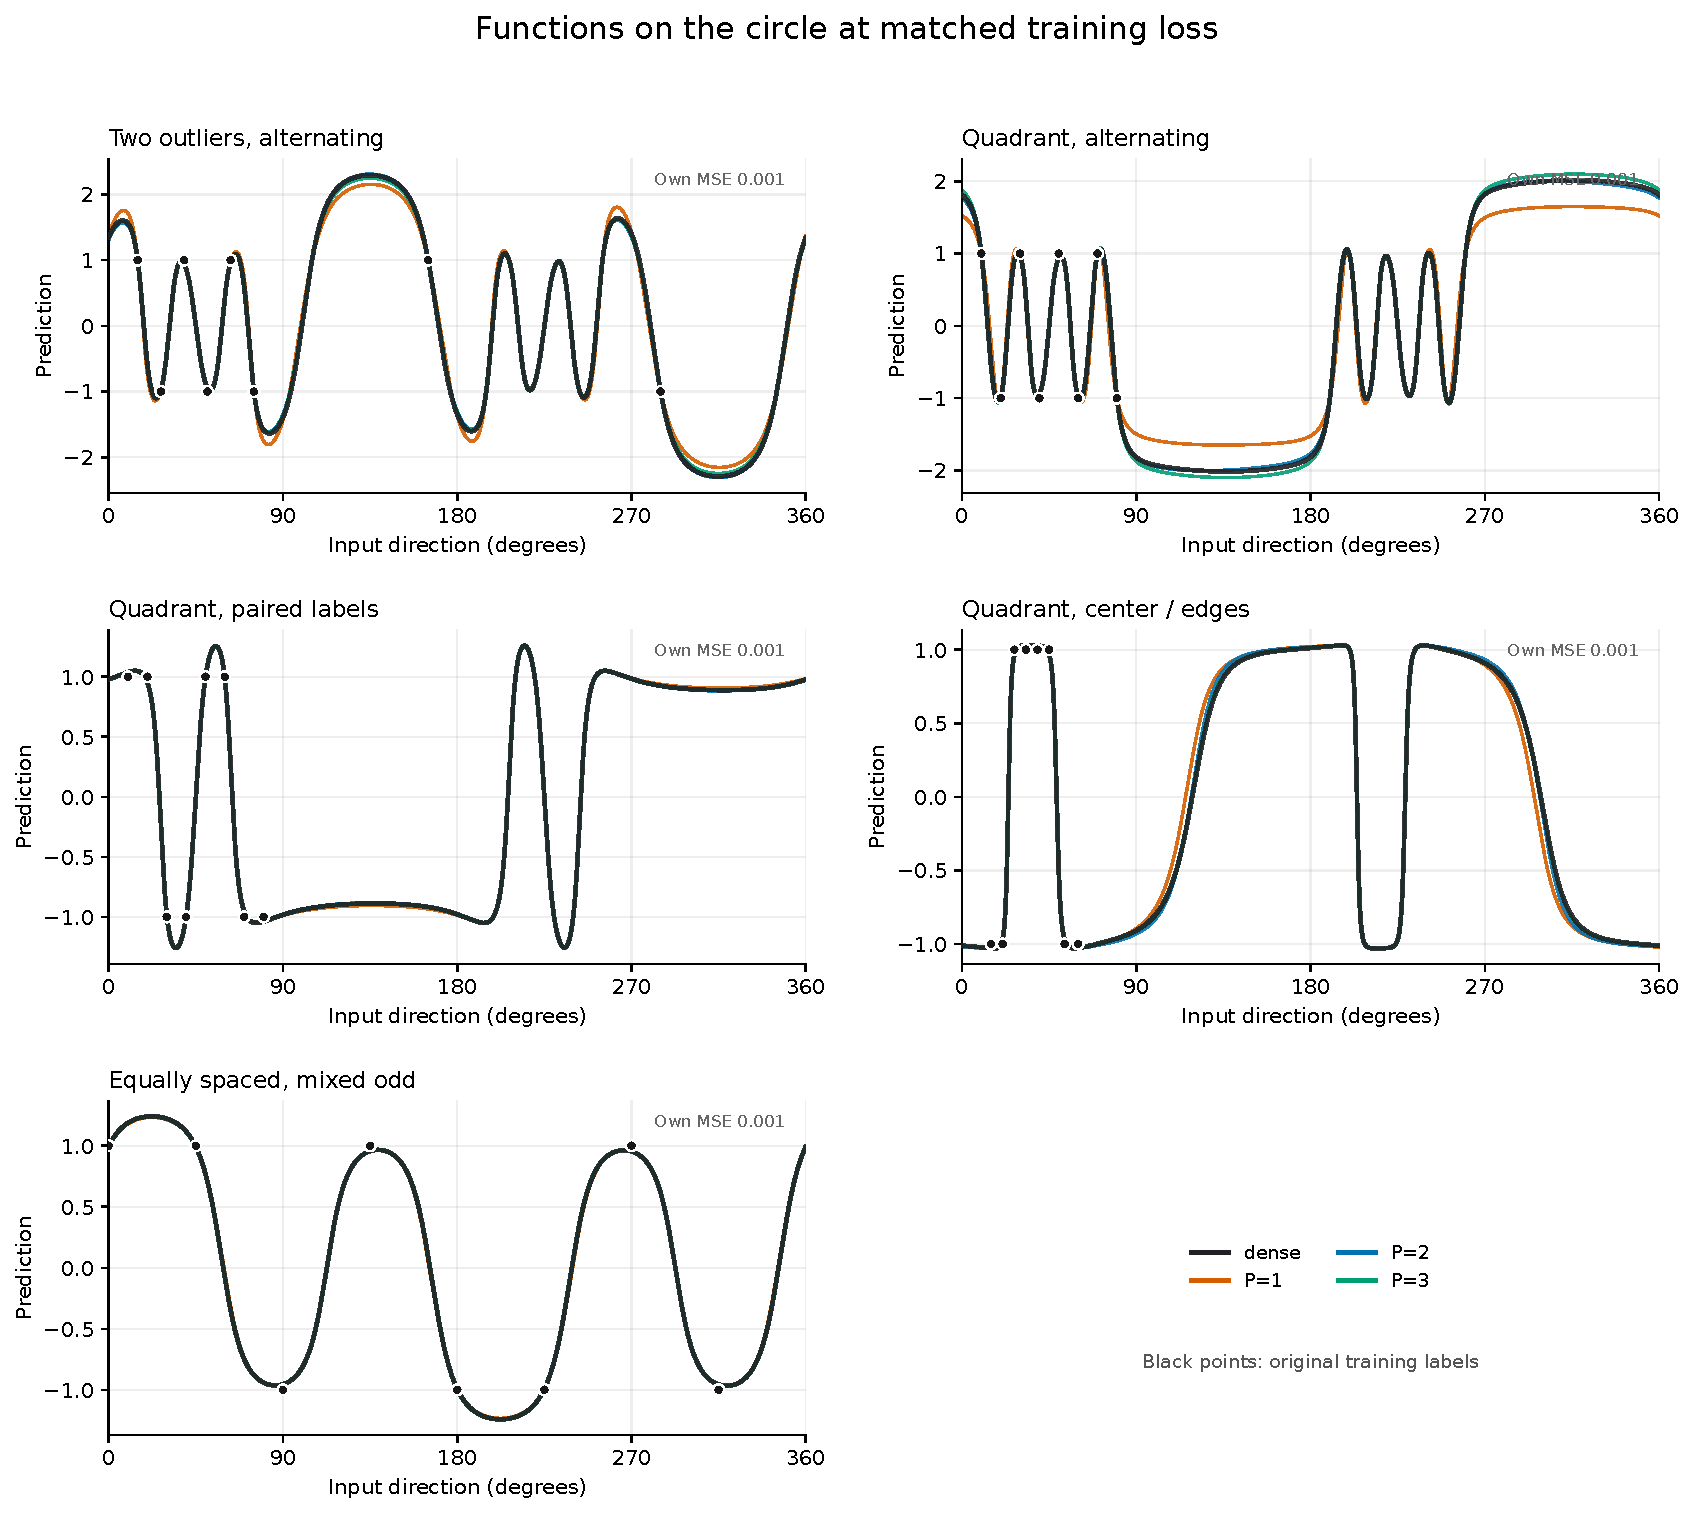
\includegraphics[width=0.86\textwidth]{figures/circle_deep.pdf}
 \caption{Three hidden tanh layers, width $4096$.  Black: dense gradient flow;
 colours: response memory of order $P=1,2,3$; dots: training labels.}
 \label{fig:deep}
\end{figure}

\begin{table}[t]
\centering
\small
\caption{Whole-circle RMS difference between response memory and dense
gradient flow.  Left: two hidden tanh layers, width $2048$.  Right: three hidden
tanh layers, width $4096$ (\Cref{fig:deep}).}
\label{tab:circle}
\begin{tabular}{lrrr@{\qquad}rrr}
\toprule
 & \multicolumn{3}{c}{two layers} & \multicolumn{3}{c}{three layers}\\
Task & $P=1$ & $P=3$ & $P=7$ & $P=1$ & $P=2$ & $P=3$\\
\midrule
Two outliers, alternating & 0.236 & 0.0730 & 0.00466 & 0.108 & 0.0238 & 0.0315\\
Quadrant, alternating & 0.341 & 0.0456 & 0.00155 & 0.275 & 0.0284 & 0.0585\\
Quadrant, paired & 0.0193 & 0.00282 & 0.00012 & 0.0122 & 0.00371 & 0.00121\\
Quadrant, center/edges & 0.0456 & 0.00488 & 0.00131 & 0.0790 & 0.0257 & 0.00725\\
Equally spaced, mixed & 0.0124 & 0.00053 & $4\times10^{-6}$ & 0.0150 & 0.00241 & 0.00028\\
\bottomrule
\end{tabular}
\end{table}

\begin{figure}[t]
 \centering
 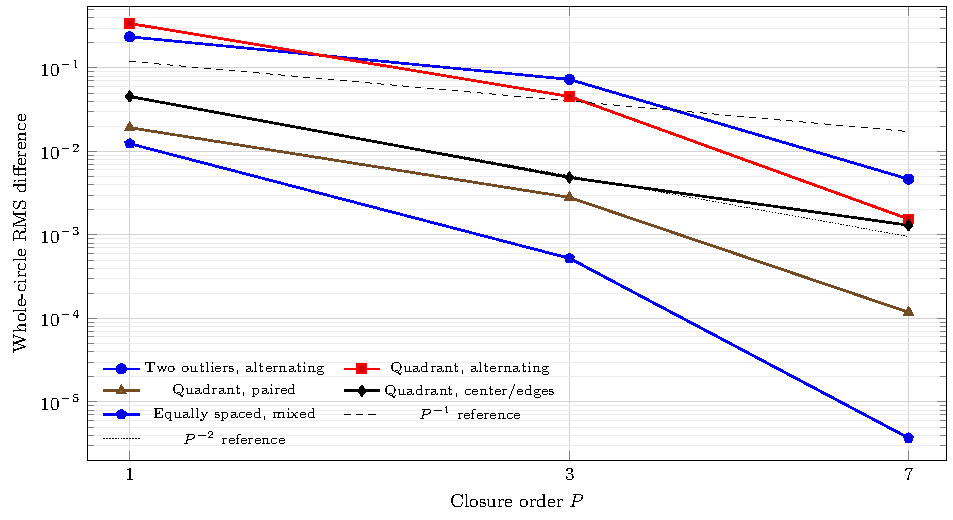
\includegraphics[width=0.55\textwidth]{figures/order_decay.pdf}
 \caption{Whole-circle difference from dense training against order, two hidden
 tanh layers (left half of \Cref{tab:circle}), with reference slopes.  These are
 matched-loss discrepancies of fitted functions, not the same-time trajectory
 error bounded by \Cref{thm:old}.}
 \label{fig:order}
\end{figure}

\paragraph{Circle tasks.}
In two layers the error falls by 1.5--3 orders of magnitude from $P=1$ to $P=7$
on every task, faster than the $P^{-1}$ trajectory bound (\Cref{fig:order}); the
theorem is an upper bound on a different quantity, and we do not read a rate off
these five points.  In three layers $P=2$ and $P=3$ stay within $0.06$ of the dense
function everywhere, and within $0.01$ on three tasks, while the hidden layers
move substantially: relative activation displacement is $0.35$--$0.65$,
$0.38$--$0.74$ and $0.46$--$0.68$ in the three layers.  Order is not monotone at
fixed width: $P=2$ beats $P=3$ on both alternating tasks.  The moving state at
$P=3$ is about $3$\,MiB against $256$\,MiB for the dense learned matrices.

\paragraph{Evolving memories versus fixed or trained bases.}
The corollary says that learned increments are low-rank \emph{in their own
history}.  Other low-rank bases do not work.  Frozen dictionaries built at initialization reach RMS $0.55$--$1.38$ on the
outlier task with about 45 vectors, against $0.073$ for 48 response moments.  A
directly trained low-rank correction of the middle matrix, with factors of
matched rank and the same $W_0^{(2)}$, lost in all 29 valid comparisons, 28 of
them by more than a factor of two; at rank 56 on the outlier task the errors were
$0.0047$ against $0.52$ and $0.25$ for two factor seeds.

\begin{figure}[t]
 \centering
 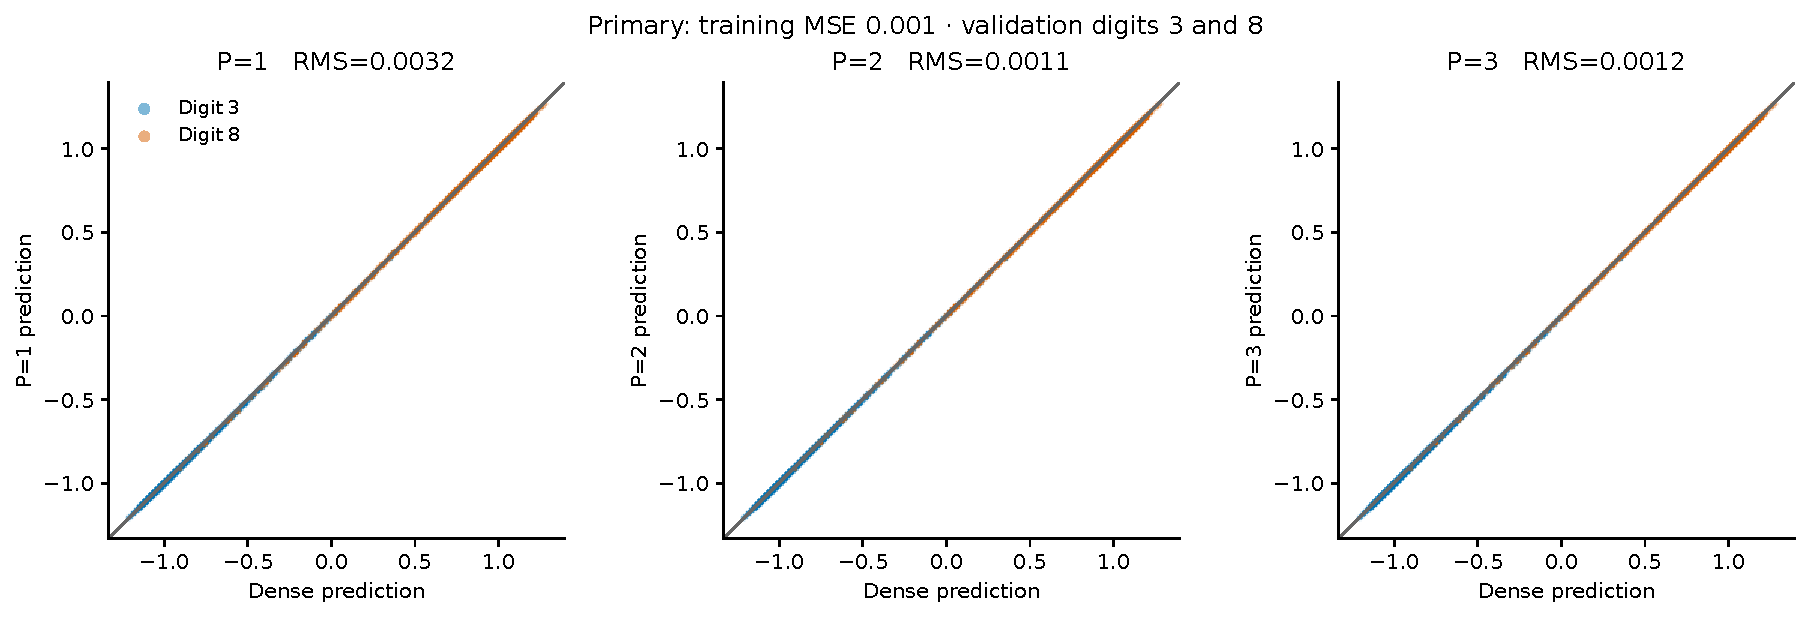
\includegraphics[width=\textwidth]{figures/mnist_scatter.pdf}
 \caption{MNIST 3 versus 8, 100 training images, width $4096$: response memory
 versus dense predictions on 1984 held-out images.  RMS differences are
 $0.0032$, $0.0011$ and $0.0012$ for $P=1,2,3$.}
 \label{fig:mnist}
\end{figure}

\paragraph{MNIST.}
Predictions of response memory and dense training on held-out images lie on the
diagonal (\Cref{fig:mnist}), with identical test accuracy ($94.7\%$).  With 1000
training images and width $1024$ the differences are $0.019$, $0.0019$ and
$0.0012$ for $P=1,2,3$, with $97.5\%$ accuracy for dense, $P=2$ and $P=3$.

\paragraph{Two clocks.}
The joint clock's better rate is asymptotic.  At $P=5$ it improved some cases
(tanh alternating quadrant $0.0066\to0.0035$; GELU outliers $0.0020\to0.0010$)
and was much worse on another (GELU alternating quadrant $0.013\to1.00$, reduced
to $0.10$ by halving the step).  Over an 82-configuration sweep, on the 65
configurations where dense and all orders fit, the joint clock's median
differences were $0.031$, $0.013$ and $0.0066$ for $P=1,2,3$.

\section{Discussion: toward an idealized model of learning}

We asked whether the idealized limit of deep feature learning can be described
by a small state, in the way a large physical system is described by a few
collective variables.  Exactly, the evidence says no: autonomous exact
descriptions appear to require operators or infinite hierarchies, and simple
scalar closures fail.  Approximately, a different kind of compression appears.
The known exact descriptions compress width and keep the whole history; we keep
the neurons and compress the history.  Measured in a clock that follows learning,
the memory of deep nonlinear feature learning is summarized by a few moments per
neuron and sample, with an error that decreases polynomially in the number of
moments and a state that does not grow with training time.  The closest
historical analogue is the moment closure of kinetic theory, where a few moments
of a distribution replace its full evolution; such closures are usually adopted
without convergence guarantees, whereas here the truncation comes with a rate.

Seen from far enough away, every description of training that keeps depth,
nonlinearity and feature learning pays for the limit in some currency and buys
accuracy with the matching knob: the network in neurons, the exact limits in
stored history, the tangent hierarchy in tensors over tuples of samples, and
response memory in an approximation order.  Descriptions that give up one of
the three are not on this axis at all; they are exact about a different object.
Stated this way, the axis is a definition and a classification
(\Cref{def:size}, \Cref{tab:axis}), not a ranking.  What the present results
add to it is one fact: at fixed width, response memory is the only description
we know of whose evolving state is set by an order rather than by the elapsed
steps or by the sample combinatorics, and whose error is certified against the
full trajectory (\Cref{sec:size}).  Whether the same holds against the
population flow is exactly \Cref{conj:population}.  \Cref{app:size} works out,
under stated hypotheses, what each description would cost at a prescribed
accuracy; the reader should take those exponents as the shape of a trade-off
rather than as a verdict, for three reasons.  The comparison identifies gradient
descent with gradient flow.  Several of the descriptions, ours included at the
population level, do not prove existence of the limit they describe.  And our
constants have no proven growth law in the horizon or the width, so ``constant
in time'' is a statement about the state, not about the constants.

The variables that survive are \emph{neuron-level memory variables}: for each
neuron and sample, compressed summaries of how it has responded forward and
backward, coupled through a fixed random operator.  They become collective only
at the population level, and \Cref{conj:population} states what that would
require.  Other gaps remain.  The initialized random operator $W_0$ is kept
exactly; it plays the role of a fixed random environment, and compressing it
while preserving its forward and adjoint reuse is the main open problem.  The
constants depend on width and horizon, and the small orders that work in
practice are not explained by the asymptotic rates.  We have not ablated the
clock against physical time.  Finally, the theory covers smooth activations, and
the memory grows with the number of training samples, so learning over a
continuum of inputs needs a further representation of the input dependence.

\begin{thebibliography}{15}
\providecommand{\natexlab}[1]{#1}
\providecommand{\url}[1]{\texttt{#1}}
\expandafter\ifx\csname urlstyle\endcsname\relax
  \providecommand{\doi}[1]{doi: #1}\else
  \providecommand{\doi}{doi: \begingroup \urlstyle{rm}\Url}\fi

\bibitem[Bordelon and Pehlevan(2022)]{bordelon2022dmft}
Blake Bordelon and Cengiz Pehlevan.
\newblock Self-consistent dynamical field theory of kernel evolution in wide
  neural networks, 2022.
\newblock URL \url{https://arxiv.org/abs/2205.09653}.

\bibitem[Bordelon and Pehlevan(2023)]{bordelon2023finite}
Blake Bordelon and Cengiz Pehlevan.
\newblock Dynamics of finite width kernel and prediction fluctuations in mean
  field neural networks, 2023.
\newblock URL \url{https://arxiv.org/abs/2304.03408}.

\bibitem[Chizat and Bach(2018)]{chizat2018global}
L{\'e}na{\"i}c Chizat and Francis Bach.
\newblock On the global convergence of gradient descent for over-parameterized
  models using optimal transport.
\newblock In \emph{Advances in Neural Information Processing Systems},
  volume~31, 2018.

\bibitem[Chizat et~al.(2024)Chizat, Colombo, Fern\'andez-Real, and
  Figalli]{chizat2024linear}
L{\'e}na{\"i}c Chizat, Maria Colombo, Xavier Fern\'andez-Real, and Alessio
  Figalli.
\newblock Infinite-width limit of deep linear neural networks.
\newblock \emph{Communications on Pure and Applied Mathematics}, 2024.
\newblock \doi{10.1002/cpa.22200}.

\bibitem[Chizat et~al.(2019)Chizat, Oyallon, and Bach]{chizat2019lazy}
L{\'e}na{\"i}c Chizat, Edouard Oyallon, and Francis Bach.
\newblock On lazy training in differentiable programming.
\newblock In \emph{Advances in Neural Information Processing Systems},
  volume~32, 2019.

\bibitem[Fang et~al.(2020)Fang, Lee, Yang, and Zhang]{fang2020features}
Cong Fang, Jason~D. Lee, Pengkun Yang, and Tong Zhang.
\newblock Modeling from features: A mean-field framework for over-parameterized
  deep neural networks, 2020.
\newblock URL \url{https://arxiv.org/abs/2007.01452}.

\bibitem[Gu et~al.(2020)Gu, Dao, Ermon, Rudra, and R{\'e}]{gu2020hippo}
Albert Gu, Tri Dao, Stefano Ermon, Atri Rudra, and Christopher R{\'e}.
\newblock {HiPPO}: Recurrent memory with optimal polynomial projections, 2020.
\newblock URL \url{https://arxiv.org/abs/2008.07669}.

\bibitem[Huang and Yau(2020)]{huang2020nth}
Jiaoyang Huang and Horng-Tzer Yau.
\newblock Dynamics of deep neural networks and neural tangent hierarchy, 2020.
\newblock URL \url{https://arxiv.org/abs/1909.08156}.

\bibitem[Jacot et~al.(2018)Jacot, Gabriel, and Hongler]{jacot2018ntk}
Arthur Jacot, Franck Gabriel, and Cl{\'e}ment Hongler.
\newblock Neural tangent kernel: Convergence and generalization in neural
  networks, 2018.
\newblock URL \url{https://arxiv.org/abs/1806.07572}.

\bibitem[Lee et~al.(2019)Lee, Xiao, Schoenholz, Bahri, Novak, Sohl-Dickstein,
  and Pennington]{lee2019wide}
Jaehoon Lee, Lechao Xiao, Samuel~S. Schoenholz, Yasaman Bahri, Roman Novak,
  Jascha Sohl-Dickstein, and Jeffrey Pennington.
\newblock Wide neural networks of any depth evolve as linear models under
  gradient descent, 2019.
\newblock URL \url{https://arxiv.org/abs/1902.06720}.

\bibitem[Mei et~al.(2018)Mei, Montanari, and Nguyen]{mei2018meanfield}
Song Mei, Andrea Montanari, and Phan-Minh Nguyen.
\newblock A mean field view of the landscape of two-layer neural networks,
  2018.
\newblock URL \url{https://arxiv.org/abs/1804.06561}.

\bibitem[Nguyen and Pham(2023)]{nguyen2023rigorous}
Phan-Minh Nguyen and Huy~Tuan Pham.
\newblock A rigorous framework for the mean field limit of multilayer neural
  networks.
\newblock \emph{Mathematical Statistics and Learning}, 6\penalty0
  (3/4):\penalty0 201--357, 2023.
\newblock \doi{10.4171/MSL/42}.

\bibitem[Saxe et~al.(2014)Saxe, McClelland, and Ganguli]{saxe2014exact}
Andrew~M. Saxe, James~L. McClelland, and Surya Ganguli.
\newblock Exact solutions to the nonlinear dynamics of learning in deep linear
  neural networks.
\newblock In \emph{International Conference on Learning Representations}, 2014.

\bibitem[Sirignano and Spiliopoulos(2019)]{sirignano2019lln}
Justin Sirignano and Konstantinos Spiliopoulos.
\newblock Mean field analysis of neural networks: A law of large numbers, 2019.
\newblock URL \url{https://arxiv.org/abs/1805.01053}.

\bibitem[Yang and Hu(2021)]{yang2021tensor}
Greg Yang and Edward~J. Hu.
\newblock Tensor programs {IV}: Feature learning in infinite-width neural
  networks.
\newblock In \emph{Proceedings of the 38th International Conference on Machine
  Learning}, volume 139 of \emph{Proceedings of Machine Learning Research},
  pages 11727--11737. PMLR, 2021.
\newblock URL \url{https://proceedings.mlr.press/v139/yang21c.html}.

\bibitem[Zhao et~al.(2023)Zhao, Zhang, Chen, Sch{\"a}fer, and
  Anandkumar]{zhao2023inrank}
Jiawei Zhao, Yifei Zhang, Beidi Chen, Florian Sch{\"a}fer, and Anima
  Anandkumar.
\newblock {InRank}: Incremental low-rank learning, 2023.

\end{thebibliography}

\appendix

\section{\texorpdfstring{Proof of \Cref{thm:old}}{Proof of the learning-speed clock theorem}}
\label{app:proof-old}

Throughout the appendices we write $b^{(\ell)}_a=r_a\delta^{(\ell)}_a/\rho$ for the
residual-weighted backward response, $\bar h^{(\ell-1)}_a$ and $\bar b^{(\ell)}_a$
for its and the forward response's histories in the clock coordinate $\xi$
(extended over the unit prefix as in the main text), and $h^{(\ell-1)*}_a$,
$b^{(\ell)*}_a$ for the values at the current endpoint of their degree-$(P-1)$
Legendre projections.  The only approximation-theoretic input is the following
Legendre tail bound.

\begin{lemma}[Legendre tail]
\label{lem:legendre}
For $q\in H^1(0,\tau;\R^N)$,
\begin{equation}
 \norm{q-\Pi_Pq}_{L^2(0,\tau)}^2
 \le\frac{1}{P(P+1)}\int_0^\tau \xi(\tau-\xi)
 \norm{q'(\xi)}^2\dd\xi
 \le\frac{\tau^2}{4P(P+1)}\norm{q'}_{L^2(0,\tau)}^2. \label{eq:leg-tail}
\end{equation}
\end{lemma}

\begin{proof}
On $[0,1]$, the shifted Legendre equation is
\[
 -\frac{\dd}{\dd x}\{x(1-x)p_k'(x)\}=k(k+1)p_k(x).
\]
Integration by parts shows that the derivatives are orthogonal in the weight
$x(1-x)$ and have squared norm $k(k+1)/(2k+1)$.  Applying Bessel's inequality
to $q'$ in this weighted space gives
\[
 \sum_{k\ge1}k(k+1)\frac{\norm{c_k}^2}{2k+1}
 \le\int_0^1x(1-x)\norm{q'(x)}^2\dd x,
\]
where $c_k=(2k+1)\int_0^1q(x)p_k(x)\dd x$.  Parseval, polynomial density and
$k(k+1)\ge P(P+1)$ for $k\ge P$ give the first bound on $[0,1]$.
Rescaling and $\xi(\tau-\xi)\le\tau^2/4$ give
\eqref{eq:leg-tail}; summing componentwise proves the vector statement.
\end{proof}

\paragraph{Step 1: dense existence and a common compact region.}
The mobility matrix $\mathcal D$ has largest eigenvalue $n$, and
$F=-\mathcal D\nabla\cL$.  Hence
\begin{equation}
 \dot\cL=-\norm{\mathcal D^{-1/2}\dot\theta}^2,
 \qquad \int_0^t\norm{\dot\theta(s)}^2\dd s\le n\rho(0)^2. \label{eq:energy}
\end{equation}
Thus $\norm{\theta(t)-\theta(0)}\le\sqrt{nt}\rho(0)$.  A finite maximal
endpoint would have a finite limiting state, from which local existence would
extend the solution, so the dense flow is global.

Now fix $T$ and let
\[
 R=\norm{\theta(0)}+\sqrt{nT}\rho(0)+1,
 \qquad \mathcal B=\{\vartheta:\norm{\vartheta}\le R\}.
\]
The dense path stays at distance at least one from $\partial\mathcal B$.  We
stop the closure at its first exit from $\mathcal B$; the rest of the proof uses
constants on this explicit ball and eventually rules out that exit.

To make the constants concrete, set $X=\max_a\norm{x_a}/\sqrt d$ and $\alpha_0=X$, and
choose recursively
\begin{align}
 s_\ell&=\sup_{|z|\le R\alpha_{\ell-1}}|\phi'(z)|,&
 \alpha_\ell&=\sqrt n\sup_{|z|\le R\alpha_{\ell-1}}|\phi(z)|,\nonumber\\
 \beta_H&=R s_H,& \beta_\ell&=s_\ell R\beta_{\ell+1}\quad(\ell<H).
                                                               \label{eq:response-bounds}
\end{align}
Then $\norm{h_a^{(\ell)}}\le\alpha_\ell$ and
$\norm{\delta_a^{(\ell)}}\le\beta_\ell$ on $\mathcal B$.  Put
\begin{align}
 Y&=\left(m^{-1}\sum_a y_a^2\right)^{1/2},&
 q&=R\alpha_H/n+Y,& S&=Tq,& \mathsf A&=1+S,\nonumber\\
 v_1&=2\beta_1X,&
 v_\ell&=2\beta_\ell\alpha_{\ell-1}/n,& v_w&=2\alpha_H,\nonumber\\
 V&=\left(v_1^2+\sum_{\ell=2}^Hv_\ell^2+v_w^2\right)^{1/2}. \label{eq:compact-constants}
\end{align}
On the stopped interval, $\rho\le q$, $\tau\le\mathsf A$ and
$\norm{F}\le V\rho$.  Since $F$ is locally Lipschitz, it has some finite
Lipschitz constant $K$ on $\mathcal B$.

\paragraph{Step 2: an exact projection-error energy.}
For any single forward or backward history $q$, let
$D_q(t)=\norm{q-\Pi_Pq}_{L^2(0,\tau(t))}^2$, and let $q^*$ be the polynomial
projection evaluated at the current endpoint.  Differentiating the raw energy
and the projected energy with \eqref{eq:old-ode}, every basis-dilation term
cancels, leaving
\begin{equation}
 \dot D_q=\rho\norm{q-q^*}^2,
 \qquad D_q(t)=\int_0^t\rho(s)\norm{q(s)-q^*(s)}^2\dd s. \label{eq:projection-energy}
\end{equation}
The jump at the end of the backward prefix is harmless, since only square
integrability and growing integrals are used.

Next differentiate \eqref{eq:old-recon}.  The physical closure equation is
exactly
\begin{equation}
 \dot{\widehat\theta}_P=F(\widehat\theta_P)+E,\qquad E_1=E_w=0,
\end{equation}
with internal defects
\begin{equation}
 E_\ell=\frac{2\rho}{nm}\sum_a
 (b^{(\ell)}_a-b^{(\ell)*}_a)(h^{(\ell-1)}_a-h^{(\ell-1)*}_a)^\top. \label{eq:defect}
\end{equation}
The two mixed projection terms vanish by orthogonality, so the defect is a pure
product of errors.  Consequently
\begin{equation}
 \int_0^t\norm{E_\ell(s)}_F\dd s
 \le\frac{2}{nm}\sum_a\sqrt{D_{b,\ell,a}(t)D_{h,\ell,a}(t)}. \label{eq:defect-energy}
\end{equation}
This inequality is the bridge from a same-history approximation bound to a
trajectory theorem.  Define also the proof-only accumulator
\[
 W^{(\ell)}_{\rm acc}(t)=W_0^{(\ell)}
 -\frac{2}{nm}\sum_a\int_0^t
 \widehat r_a\widehat\delta_a^{(\ell)}
 (\widehat h_a^{(\ell-1)})^\top\dd s,\qquad
 R_\ell=\widehat W^{(\ell)}-W^{(\ell)}_{\rm acc}.
\]
Then $R_\ell(0)=0$ and $\dot R_\ell=E_\ell$, so \eqref{eq:defect-energy}
controls the accumulated absolute velocity error, not only a signed endpoint
integral.

\paragraph{Step 3: forward histories have a $P$-independent derivative bound.}
Before changing variables, note that a nonstationary learning-speed solution
cannot first reach $\rho=0$ at a finite regular state.  Every raw velocity
vanishes there, and local uniqueness applied backward from that equilibrium
would force the preceding path to be stationary.  Hence $\xi=\tau(t)$ is a
valid coordinate on every nonstationary compact segment; the raw algorithm
itself remains defined at $\rho=0$ without division.

Write primes for derivatives in $\xi=\tau(t)$ and define
\[
 Z_\ell(t)=\frac1m\sum_a\int_0^{\tau(t)}
 \norm{(h_a^{(\ell)})'(\xi)}^2\dd\xi.
\]
The first layer satisfies $\norm{(h_a^{(1)})'}\le s_1v_1X$.  For later layers,
the chain rule gives
\begin{equation}
 (h_a^{(\ell)})'=\phi'(z_a^{(\ell)})\od
 \left[(F_\ell/\rho+E_\ell/\rho)h_a^{(\ell-1)}
 +\widehat W^{(\ell)}(h_a^{(\ell-1)})'\right].       \label{eq:forward-chain}
\end{equation}
The delicate term is the defect, because endpoint evaluation of a polynomial
projection can amplify errors by a factor that grows with $P$.  Endpoint
evaluation of a degree-$(P-1)$ polynomial has operator norm $P/\sqrt\tau$ from
$L^2(0,\tau)$, because $\sum_{k<P}(2k+1)=P^2$.  Projection contraction and
$m^{-1}\sum_a\norm{b^{(\ell)}_a}^2\le\beta_\ell^2$ then imply
\[
 \left(m^{-1}\sum_a\norm{b^{(\ell)*}_a}^2\right)^{1/2}\le P\beta_\ell,
 \quad
 \left(m^{-1}\sum_a\norm{b^{(\ell)}_a-b^{(\ell)*}_a}^2\right)^{1/2}
 \le(P+1)\beta_\ell.
\]
Combining this with \Cref{lem:legendre}, \eqref{eq:projection-energy} and
\eqref{eq:defect} yields
\begin{equation}
 \int_0^t\rho\norm{E_\ell/\rho}_F^2\dd s
 \le\frac{2\beta_\ell^2\mathsf A^2}{n^2}
 Z_{\ell-1}(t).                                      \label{eq:e-square}
\end{equation}
Here the endpoint factor $P+1$ cancels the $P^{-1}$ projection factor.  This
cancellation is the step that prevents a loss of convergence order with depth.

Define finite, $P$-independent bounds recursively by
\begin{align}
 \overline Z_1&=S(s_1v_1X)^2,\nonumber\\
 \overline Z_\ell&=3s_\ell^2\left[
 S v_\ell^2\alpha_{\ell-1}^2+
 \left(R^2+\frac{2\beta_\ell^2\mathsf A^2\alpha_{\ell-1}^2}{n^2}\right)
 \overline Z_{\ell-1}\right].                       \label{eq:z-recursion}
\end{align}
Integrating \eqref{eq:forward-chain}, and using
$\norm{x+y+z}^2\le3(\norm{x}^2+\norm{y}^2+\norm{z}^2)$ together with
\eqref{eq:e-square}, proves inductively that $Z_\ell\le\overline Z_\ell$.

\paragraph{Step 4: accumulated defect and feedback.}
The zero backward prefix gives $m^{-1}\sum_aD_{b,\ell,a}\le S\beta_\ell^2$, and
\Cref{lem:legendre} gives
\[
 \frac1m\sum_aD_{h,\ell,a}
 \le\frac{\mathsf A^2\overline Z_{\ell-1}}{4P(P+1)}.
\]
Summing \eqref{eq:defect-energy} over links, we obtain
\begin{equation}
 \int_0^t\norm{E(s)}\dd s
 \le\frac{B_{\mathrm{LS}}}{\sqrt{P(P+1)}},\qquad
 B_{\mathrm{LS}}=\frac{\mathsf A}{n}
 \sum_{\ell=2}^H\beta_\ell\sqrt{S\overline Z_{\ell-1}}. \label{eq:old-defect-bound}
\end{equation}
It remains to account for feedback.  Subtracting the dense flow from the
perturbed flow and applying the Lipschitz bound on $F$ gives
\[
 e(t)\le\frac{B_{\mathrm{LS}}}{\sqrt{P(P+1)}}
 +K\int_0^te(s)\dd s,
\]
and Gronwall's inequality yields
\begin{equation}
 \sup_{t\le T}e(t)\le
 \frac{B_{\mathrm{LS}}e^{KT}}{\sqrt{P(P+1)}}.       \label{eq:old-explicit}
\end{equation}
Choose $P_0$ so that the right side is less than $1/2$.  The closure then
cannot reach $\partial\mathcal B$.  Its moment representations,
$1\le\tau\le\mathsf A$ and the response bounds place its whole finite state in a
compact subset of the locally Lipschitz domain.  A finite maximal endpoint would
therefore extend, so the closure exists through $T$.  Lipschitz dependence of
the network responses on $\theta$ gives the final prediction statement.

\paragraph{Globally bounded activations.}
Suppose now that every activation and its first derivative are globally
bounded.  Set
\[
 \alpha_\ell=\sqrt n\norm{\phi}_\infty,\qquad
 s_\ell=\norm{\phi'}_\infty,\qquad
 B_w=\sqrt{\norm{w(0)}^2+nY^2T}.
\]
For both the dense and the closure flows, the unchanged readout equation obeys
\[
 \frac{\dd}{\dd t}\norm w^2
 =nY^2-4n\frac1m\sum_a(f_a-y_a/2)^2\le nY^2.
\]
Therefore $\norm w\le B_w$, $\rho\le q:=B_w\alpha_H/n+Y$, $S=Tq$ and
$\tau\le\mathsf A:=1+S$.  Start with $\beta_H=B_ws_H$ and proceed downward: for
$\ell=H,\ldots,2$, define
\[
 D_\ell=\norm{W_0^{(\ell)}}_F+
 \frac{2\mathsf A\beta_\ell\alpha_{\ell-1}}{n},
 \qquad \beta_{\ell-1}=s_{\ell-1}D_\ell\beta_\ell.
\]
Projection contraction in \eqref{eq:projection-form} gives
$\norm{\widehat W^{(\ell)}}_F\le D_\ell$, and the backward recurrence then gives
$\norm{\delta^{(\ell-1)}}\le\beta_{\ell-1}$.  There is no circularity, because
the descent starts from the bounded readout.  Finally,
\[
 \norm{W^{(1)}(t)}_F\le\norm{W^{(1)}(0)}_F+2SX\beta_1.
\]
These $P$-independent physical bounds, the moment integral representations and
$1\le\tau\le\mathsf A$ place the order-$P$ state in a compact set for every
fixed $P$, so the closure continues through $T$ for every $P\ge1$.  Repeating
Steps 2--4 with these global constants gives \eqref{eq:old-explicit} for every
$P$.  This completes the proof. \qed


\section{\texorpdfstring{The joint feature-learning clock: construction and proof of \Cref{thm:new}}{The joint feature-learning clock: construction and proof}}
\label{app:proof-new}

\paragraph{Construction.}
Let $\Psi$ be the concatenation over $\ell\ge2$ and $a$ of the forward and
residual-weighted backward responses $(h^{(\ell-1)}_a,b^{(\ell)}_a)$, so that the
clock \eqref{eq:new-clock} reads $\dot\tau=g=\rho+\norm{\dot\Psi}_2$ and
$\norm{\dd\Psi/\dd\tau}\le1$.  History is placed at $\xi=\tau(s)$ with mass
$\rho(s)\dd s$, while the prefix $[0,1]$ carries Lebesgue mass and constant
initial responses; the resulting measure $\mu_t$ satisfies $\dd\mu_t\le\dd\xi$.
With $p=(p_0,\ldots,p_{P-1})^\top$ evaluated at $\xi/\tau$, $e=(1,\ldots,1)^\top$,
and the triangular matrix $\mathsf T_{kk}=k$, $\mathsf T_{kj}=2j+1$ for $j<k$
(zero above the diagonal), the state consists of the moment matrices
$\bar h^{(\ell-1)}_a=\int\bar h^{(\ell-1)}_a(\xi)\,p^\top\dd\mu_t$,
$\bar\delta^{(\ell)}_a=\int\bar b^{(\ell)}_a(\xi)\,p^\top\dd\mu_t$ and one shared
Gram matrix $G=\int pp^\top\dd\mu_t$, which evolve by
\begin{align}
 \widehat W^{(\ell)}&=W_0^{(\ell)}-\frac{2}{nm}\sum_a
 \bigl(\bar\delta^{(\ell)}_aG^{-1}(\bar h^{(\ell-1)}_a)^\top
 -b^{(\ell)}_a(0)\,h^{(\ell-1)}_a(0)^\top\bigr),\nonumber\\
 \dot{\bar h}^{(\ell-1)}_a&=\rho\,h^{(\ell-1)}_ae^\top-(g/\tau)\,\bar h^{(\ell-1)}_a\mathsf T^\top,
 \qquad
 \dot{\bar\delta}^{(\ell)}_a=r_a\delta_a^{(\ell)}e^\top-(g/\tau)\,\bar\delta^{(\ell)}_a\mathsf T^\top,
 \nonumber\\
 \dot G&=\rho\,ee^\top-(g/\tau)(\mathsf TG+G\mathsf T^\top),     \label{eq:new-ode}
\end{align}
with $G(0)=\diag(1,\tfrac13,\ldots,\tfrac1{2P-1})$, only the zeroth moment
columns nonzero initially, and the prefix product subtracted so that
$\widehat W^{(\ell)}(0)=W_0^{(\ell)}$.  With $h^{(\ell-1)*}_a=\bar h^{(\ell-1)}_aG^{-1}e$
and $b^{(\ell)*}_a=\bar\delta^{(\ell)}_aG^{-1}e$, differentiating the
reconstruction cancels every $g/\tau$ term and gives the defect
$E_\ell=\frac{2\rho}{nm}\sum_a(b^{(\ell)}_a-b^{(\ell)*}_a)(h^{(\ell-1)}_a-h^{(\ell-1)*}_a)^\top$,
of the same product form as \eqref{eq:defect}.


\paragraph{Step 1: a lower bound on the dense residual.}
Assume $\rho_0>0$ as stated, and use the compact physical ball $\mathcal B$ from
\Cref{app:proof-old}.  Retain the constants
$\alpha_\ell,\beta_\ell,q,S,\mathsf A,V,K$ from the proof of \Cref{thm:old}.  On
this ball the output map has a finite Lipschitz constant $c_f$: prediction and
residual RMS change by at most $c_f\norm{\theta-\theta'}$.  Along dense flow,
\[
 |\dot\rho_{\rm dense}|\le c_f\norm{F(\theta)}
 \le c_fV\rho_{\rm dense}.
\]
Consequently
\begin{equation}
 \rho_{\rm dense}(t)\ge
 \mu:=\rho_0e^{-c_fVT}>0,\qquad 0\le t\le T.          \label{eq:dense-rho-lower}
\end{equation}

\paragraph{Step 2: an exact weighted projection energy.}
Consider the maximal regular closure interval stopped before either its
physical state leaves $\mathcal B$ or its residual reaches $\mu/2$.  We first
derive a clock bound on this stopped interval without assuming small projection
error.  For any inserted vector history $f$, let
\[
 D_f=\norm{f-\Pi_t f}_{L^2(\mu_t)}^2
 =\int\norm f^2\dd\mu_t-\operatorname{tr}(B_fG^{-1}B_f^\top).
\]
Differentiating $G^{-1}G=I$ gives
\[
 \frac{\dd}{\dd t}G^{-1}
 =-\rho G^{-1}ee^\top G^{-1}
 +(g/\tau)(G^{-1}\mathsf T+\mathsf T^\top G^{-1}).
\]
Together with \eqref{eq:new-ode}, this cancels every dilation term and yields
\begin{equation}
 \dot D_f=\rho\norm{f-f^*}^2,\qquad
 D_f(t)=\int_0^t\rho\norm{f-f^*}^2\dd s.             \label{eq:new-energy}
\end{equation}
The initial error is zero because every prefix is constant.  Thus
\eqref{eq:defect-energy} holds with the weighted errors in
\eqref{eq:new-energy}.

\paragraph{Step 3: order-independent coarse bounds.}
Put
\[
 Q=m\sum_{\ell=2}^H(\alpha_{\ell-1}^2+\beta_\ell^2),
 \qquad C_0=\frac{\mathsf A Q}{nm}.
\]
The total mass of $\mu_t$ is at most $\mathsf A=1+S$.  Projection error is no
larger than raw history energy, including the matching prefixes.  Applying
$2\sqrt{uv}\le u+v$ in the defect estimate gives the order-independent bounds
\begin{equation}
 \int_0^t\norm E\dd s\le C_0,\qquad
 \int_0^t\norm{\dot{\widehat\theta}}\dd s
 \le VS+C_0.                                         \label{eq:coarse-new}
\end{equation}
The second inequality uses $\dot{\widehat\theta}=F(\widehat\theta)+E$ and
$\int_0^t\norm F\dd s\le V\int_0^t\rho\dd s\le VS$.  This total-variation
estimate is stronger than bounded physical position, and it is obtained before
any clock bound.

\paragraph{Step 4: a clock bound without a cap.}
It remains to control the derivative of the normalized response map.  Let
$q_r=r/\rho\in\R^m$.  Then
\begin{equation}
 \norm{q_r}^2=m,\qquad
 Dq_r[v]=
 \left(I-\frac{q_rq_r^\top}{m}\right)\frac{Dr[v]}{\rho}. \label{eq:normalized-residual-derivative}
\end{equation}
The matrix in parentheses is an orthogonal projector, and $\rho\ge\mu/2$ on the
stopped interval.  Differentiating the forward and backward recurrences uses
only bounded physical weights and bounded first two activation derivatives on
compact preactivation intervals; the first layer uses only $\phi'$.  Hence
there is a finite, $P$-independent constant $J$ such that
\[
 \norm{D\Psi(\vartheta)}_{\rm op}\le J
\]
throughout the stopped tube.  The stated local smoothness also makes this
derivative locally Lipschitz.  Since
$\dot\Psi=D\Psi(\widehat\theta)\dot{\widehat\theta}$, \eqref{eq:coarse-new}
now gives
\begin{equation}
 \tau_P(t)=1+\int_0^t(\rho+\norm{\dot\Psi})\dd s
 \le\mathsf A+J(VS+C_0)=:\Lambda_T.                 \label{eq:new-clock-bound}
\end{equation}
No clock cap has been assumed or inserted.

\paragraph{Step 5: the sharp joint approximation estimate.}
We can now use the sharper approximation estimate.  The entire concatenated
history $\overline\Psi(\xi)$ is constant on the prefix, continuous at its join
and, on the physical history,
\[
 \norm{\partial_\xi\overline\Psi}
 =\frac{\norm{\dot\Psi}}{\rho+\norm{\dot\Psi}}\le1.
\]
Therefore $\int_0^{\tau_P}\norm{\overline\Psi'}^2\dd\xi\le \tau_P-1$.  The weighted
projection is a best approximation in $L^2(\mu_t)$, and $\dd\mu_t\le\dd\xi$, so
comparison with the ordinary Legendre projection and \Cref{lem:legendre} give
the joint bound
\begin{equation}
 \sum_{\ell,a}(D_{h,\ell,a}+D_{b,\ell,a})
 \le\frac{\tau_P^2(\tau_P-1)}{4P(P+1)}
 \le\frac{\Lambda_T^2(\Lambda_T-1)}{4P(P+1)}.       \label{eq:new-joint-tail}
\end{equation}
This is one estimate for the concatenated path; it does not introduce a
separate dimension factor per unit or layer.

\paragraph{Step 6: feedback and continuation.}
Combining \eqref{eq:defect-energy}, \eqref{eq:new-clock-bound},
\eqref{eq:new-joint-tail} and $2\sqrt{uv}\le u+v$ yields
\begin{equation}
 \int_0^t\norm E\dd s
 \le\frac{\Gamma_{\mathrm{JF}}}{P(P+1)},\qquad
 \Gamma_{\mathrm{JF}}=\frac{\Lambda_T^2(\Lambda_T-1)}{4nm}.     \label{eq:new-sharp-defect}
\end{equation}
Subtracting the dense flow and applying the Lipschitz constant $K$ and Gronwall's
inequality gives
\begin{equation}
 \norm{\widehat\theta_P(t)-\theta(t)}
 \le\frac{\Gamma_{\mathrm{JF}}e^{KT}}{P(P+1)}.                  \label{eq:new-feedback}
\end{equation}

Choose $P_0(T)$ so that, for every $P\ge P_0(T)$,
\begin{equation}
 \frac{\Gamma_{\mathrm{JF}}e^{KT}}{P(P+1)}\le\frac12,\qquad
 c_f\frac{\Gamma_{\mathrm{JF}}e^{KT}}{P(P+1)}\le\frac\mu4.      \label{eq:new-order-condition}
\end{equation}
The first inequality rules out physical exit, because the dense path stays at
distance one from $\partial\mathcal B$.  The second, together with
\eqref{eq:dense-rho-lower}, gives $\widehat\rho\ge3\mu/4>\mu/2$, ruling out
residual exit.

Finally, the matching prefix supplies, at every fixed $P$,
\begin{equation}
 G(t)\succeq\int_0^1p(\xi/\tau_P(t))p(\xi/\tau_P(t))^\top\dd\xi. \label{eq:prefix-gram}
\end{equation}
The right side is positive definite, since a zero quadratic form would make a
nonzero polynomial vanish on an interval.  Its entries vary continuously with
$\tau_P$, so on $1\le \tau_P\le\Lambda_T$ its least eigenvalue has a positive minimum
$\gamma_{P,T}$; this minimum need not be uniform in $P$.  The moment integral
representations, finite history mass, bounded responses and bounded
fixed-order polynomials then bound every raw coordinate.  Together with the
physical, residual, clock and Gram bounds, the full state lies in a compact
subset of its locally Lipschitz domain.  A finite maximal endpoint therefore
extends, which proves continuation through $T$ and completes the theorem with
$C_T=\Gamma_{\mathrm{JF}}$ and $K_T=K$. \qed


\subsection*{Implementation of the joint clock}
\label{app:joint-impl}

Equation \eqref{eq:new-clock} appears implicit only because $\dot\Psi$ is
written compactly; no nonlinear solve for $g$ is needed.  The internal
velocities do not depend on $g$, so they can be computed first.  Begin with
$q=G^{-1}e$, the endpoint fits $a^*,b^*$, and the internal velocities
\begin{equation}
 V_\ell=\dot{\widehat W}^{(\ell)}=-\frac{2\rho}{nm}\sum_a
 \left[b^{(\ell)}_a(h^{(\ell-1)*}_a)^\top+
 b^{(\ell)*}_a(h^{(\ell-1)}_a-h^{(\ell-1)*}_a)^\top\right]. \label{eq:internal-velocity}
\end{equation}
These expressions contain no $g$.  Next compute $V_1=F_1$ and $V_w=F_w$, and run
a directional forward pass,
\[
 \dot z_a^{(1)}=V_1x_a/\sqrt d,\qquad
 \dot z_a^{(\ell)}=V_\ell h_a^{(\ell-1)}+
 \widehat W^{(\ell)}\dot h_a^{(\ell-1)},\qquad
 \dot h_a^{(\ell)}=\phi'(z_a^{(\ell)})\od\dot z_a^{(\ell)},
\]
which gives $\dot r$ and $\dot\rho$.  A reverse directional pass then
differentiates the backward recurrence, using $\phi''$ for $\ell\ge2$, and
yields
\[
 \dot b^{(\ell)}_a=\frac{\dot r_a\delta_a^{(\ell)}+
 r_a\dot\delta_a^{(\ell)}}{\rho}-b^{(\ell)}_a\frac{\dot\rho}{\rho}.
\]
Only then do we evaluate $g=\rho+\norm{\dot\Psi}$ and, finally,
\eqref{eq:new-ode}.  Matrix and transpose actions use the same reconstructed
operator.  In practice one factors $G$ and solves linear systems; an explicit
inverse is unnecessary.

The joint clock is more regular in approximation coordinates, but it is not
automatically better at low order.  At $P=1$ the polynomial space consists of
constants, so changing the coordinate alone leaves the physical constant-mode
closure unchanged.  Higher orders pay for Gram solves and derivative passes,
and the theoretical constants can be large.


\section{A frozen-span closure of the population flow}
\label{app:popclosure}


This appendix records a closure of the population flow itself, for the smallest
case allowed by the contract: two hidden layers, $\phi=\tanh$, inputs on
a circle ($d=2$, $x/\sqrt d\in S^1$) with labels $|y|\le Y$.  The population state
is the first-layer weight row $W^{(1)}\in L^2(\Omega_1;\R^2)$, the readout
$w\in L^2(\Omega_2)$ and the middle operator $W^{(2)}=W^{(2)}_0+(W^{(2)}-W^{(2)}_0)$,
where $W^{(2)}_0$ is the initialized Gaussian operator and the learned part is
Hilbert--Schmidt.  The flow is \eqref{eq:dense-flow} with $\frac1m\sum_a$
replaced by integration against a training law $\mu$ on inputs and labels, and
the reverse action is always the true adjoint $(W^{(2)})^*$.  We work on
$0\le t\le T=1/200$ and on a Wasserstein neighborhood of the two-point task
$\nu_*=\tfrac12\delta_{(\sqrt2e_1,+1)}+\tfrac12\delta_{(\sqrt2e_2,-1)}$; the
neighborhood contains perturbed, nonorthogonal, nonatomic and noisy input laws,
and neither its radius nor the interval shrinks with the closure order.

\paragraph{The compressed state.}
Enumerate the finite expressions built from constants, the Gaussian initial
weights, rational affine combinations, $\sin$, $\cos$, $\phi$, bounded products,
and the initialized actions $W^{(2)}_0$ and $(W^{(2)}_0)^*$.  At order $N$ this
gives, on each population, a finite vector of \emph{observables of the
initialization}, which we normalize by a ridge-regularized Gram matrix so that
they have unit scale.  The saved state is then
\begin{itemize}
\item the joint law, on population 1, of the current first-layer weights
$W^{(1)}$, their initial values, and the $N$ observables;
\item the joint law, on population 2, of the current readout $w$ and the $N$
observables;
\item one finite matrix $M$ representing the middle-layer action
$W^{(2)}$ between the two observable vectors, initialized from $W^{(2)}_0$.
\end{itemize}
The closure evolves this state by the population flow itself, with $W^{(2)}$
replaced by the finite operator ``project onto population-1 observables, apply
$M$, expand in population-2 observables'' and $(W^{(2)})^*$ by its transpose
(details below).  It is autonomous, uses only the current state and the
training law, and is restartable from its own saved state.  Initial and current
values are stored jointly, so same-neuron quantities such as feature displacement
are genuine observables of the state.

\begin{theorem}[Autonomous population closure]
\label{thm:popclosure}
For every separately fixed training law in the stated neighborhood of $\nu_*$
and every order $N$, the closure is uniquely well posed on $[0,T]$ and
restartable from its saved state, and as $N\to\infty$ its prediction $f_N$
converges to the population prediction $f$ uniformly on $[0,T]$ and over the
whole input circle.  Every separately fixed same-population joint observation---
initial and current hidden pairs, feature displacements, forward and adjoint
actions, bounded nonlinear pushforwards and quadratic contractions---converges
uniformly on $[0,T]$ in Wasserstein distance $W_2$.
\end{theorem}

The proof (below) controls the distance between closure and
population flow through the error of the finite observable basis; unbounded
backward fields force a truncation that turns Gronwall's inequality into an
Osgood inequality, whose solution still tends to zero with the basis error.

\begin{proposition}[Both layers learn, nonlinearly]
\label{prop:featurelearning}
On a Wasserstein neighborhood of $\nu_*$ there is a common time at which both
hidden populations have strictly positive mean-square displacement of their
activations from initialization, and strictly positive nonaffinity
$\inf_{\alpha,\beta}\E|\phi(z)-\alpha z-\beta|^2$ of their preactivations.
\end{proposition}

The small-time expansion of the flow at $\nu_*$ (below) shows
that both hidden displacements are nonzero at order $t^2$, a Gaussian
preactivation has positive nonaffinity, and continuity extends both properties
to a neighborhood.  The closure therefore converges on a family where all three
properties of the introduction hold.

\paragraph{What this compresses, and why it is not the main result.}
The learned operator $W^{(2)}-W^{(2)}_0$ of the population flow is replaced by a
finite matrix between two populations: an operator ODE becomes a population ODE
plus a finite matrix.  But the matrix acts between \emph{frozen} spans of
initialization observables, so the learned middle layer can only rotate within
a span fixed at initialization, while $W^{(1)}$ and $w$ move freely.  This is a
frozen-dictionary closure of the middle layer, and it shows the characteristic
limitations of that class: convergence comes only from the spans becoming
dense, there is no rate in $N$, and the guarantee holds on a short horizon near a
reference task.  The two laws are continuum objects, so the state is not a
finite list of scalars.  The frozen-dictionary experiments of
\Cref{sec:experiments} show the same limitation at finite width, and the
response memories of \Cref{sec:memory}, whose atoms coevolve with the features,
are the answer to it.

\subsection*{Details}

\paragraph{Population flow.}
With $\phi=\tanh$, $d=2$ and inputs $x\in\sqrt2S^1$, the population fields are
$z^{(1)}(x)=W^{(1)}\cdot x/\sqrt d$, $h^{(1)}=\phi(z^{(1)})$,
$z^{(2)}(x)=W^{(2)}h^{(1)}(x)$, $h^{(2)}=\phi(z^{(2)})$,
$\delta^{(2)}(x)=w\,\phi'(z^{(2)}(x))$,
$\delta^{(1)}(x)=\phi'(z^{(1)}(x))\,(W^{(2)})^*\delta^{(2)}(x)$ and
$f(x)=\E_2[w\,h^{(2)}(x)]$; with $r=f-y$ and a training law $\mu$,
\[
 \dot W^{(1)}=-2\!\int\! r\,\delta^{(1)}\frac{x}{\sqrt d}\dd\mu,\qquad
 \dot W^{(2)}=-2\!\int\! r\,\delta^{(2)}\otimes h^{(1)}\dd\mu,\qquad
 \dot w=-2\!\int\! r\,h^{(2)}\dd\mu .
\]

\paragraph{Observables.}
Let $\psi_1\in\R^{N_1}$ and $\psi_2\in\R^{N_2}$ be the order-$N$ vectors of
initialization observables on the two populations, ridge-normalized by
$\psi_\ell\mapsto(\E_\ell[\psi_\ell\psi_\ell^\top]+2^{-N}I)^{-1/2}\psi_\ell$, so
that the projections $g\mapsto\psi_\ell^\top\E_\ell[\psi_\ell g]$ are contractions
converging strongly to the identity on the observable spaces.  The initialized
middle action is recorded in $M_0=\E_2[\psi_2\,(W_0^{(2)}\psi_1)^\top]$; the
forward and adjoint actions of $W_0^{(2)}$ on observables are drawn from one
correlated Gaussian source, which is what makes the two orientations one
operator and its adjoint.

\paragraph{Closure.}
The state is $\Law(\psi_1,W^{(1)}_0,W^{(1)})$ on population 1,
$\Law(\psi_2,w)$ on population 2, and $M\in\R^{N_2\times N_1}$, initialized with
$W^{(1)}=W^{(1)}_0$, $w=0$ and $M=M_0$.  The closure is the population flow above
with $W^{(2)}$ replaced by
\[
 W^{(2)}_Ng=\psi_2^\top M\,\E_1[\psi_1g],\qquad
 (W^{(2)}_N)^*g=\psi_1^\top M^\top\E_2[\psi_2g],
\]
\[
 \dot M=-2\!\int\! r_N\,\E_2[\psi_2\delta^{(2)}]\,\E_1[\psi_1h^{(1)}]^\top\dd\mu,
\]
so that $z^{(2)}_N(x)=\psi_2^\top M\,\E_1[\psi_1h^{(1)}(x)]$ and
$f_N(x)=\E_2[w\,h^{(2)}_N(x)]$; the weights $W^{(1)}$ and $w$ move by the flow
equations with $r_N$ and $\delta^{(1)}_N$, which transports the two laws.  The
represented operator is $W^{(2)}_N$, whose learned part is $M-M_0$ written
between observable spaces.

\paragraph{Well-posedness.}
For fixed $N$ the characteristic equations are locally Lipschitz.  The loss
obeys $\frac{d}{dt}\cL_N=-\norm{\dot W^{(1)}}_2^2-\norm{\dot M}_F^2-\norm{\dot w}_2^2$,
and $\cL_N(0)\le Y^2$ gives $\norm{w(t)}_\infty\le2Yt$,
$\norm{M(t)-M_0}_F\le2Y^2t^2$, $\norm{W^{(2)}_N(t)}_{\mathrm{op}}\le2+2Y^2t^2$ and
$\norm{W^{(1)}(t)}_2\le\sqrt2+4Y^2t^2+2Y^4t^4$, which exclude finite-time escape.
The joint laws contain the correlations between observables and current weights,
so the saved state suffices to restart.

\paragraph{Convergence.}
Place closure and population flow on common probability spaces and set
\[
 e_N=\norm{W^{(1)}_N-W^{(1)}}_2
 +\norm{(W^{(2)}_N-W^{(2)}_{N,0})-(W^{(2)}-W^{(2)}_0)}_\HS
 +\norm{w_N-w}_2 ,
\]
where $W^{(2)}_{N,0}$ is the closure's initial operator.  The basis error
\begin{align*}
 \varepsilon_N={}&\sup_{t,x}\norm{(W^{(2)}_{N,0}-W^{(2)}_0)h^{(1)}(t,x)}_2
 +\sup_{t,x}\norm{(W^{(2)}_{N,0}-W^{(2)}_0)^*\delta^{(2)}(t,x)}_2\\
 &+\sup_t\norm{\Pi_2\dot W^{(2)}(t)\Pi_1-\dot W^{(2)}(t)}_\HS,
\end{align*}
with $\Pi_\ell$ the observable projections, tends to zero by strong convergence
of the projections, compactness of the population response curves in $(t,x)$,
and density of finite-rank operators.  Forward subtraction gives, uniformly in
$x$, $\norm{h^{(1)}_N-h^{(1)}}_2\le e_N$ and
$\norm{h^{(2)}_N-h^{(2)}}_2+|f_N-f|\le C(e_N+\varepsilon_N)$.  Backward
subtraction multiplies a changed gate by an unbounded reference field; with the
exponential tail bound of the reference trajectory, truncating at level $R$
gives
\[
 e_N'\le C(1+R)(e_N+\varepsilon_N)+C\,e^{-aR}.
\]
Choosing $R=1+a^{-1}\log(1/v)$ with $v=e_N+\varepsilon_N+\eta$ yields
$v'\le Lv\log(e/v)$, hence
\[
 e_N(t)+\varepsilon_N+\eta\le e^{1-\alpha(t)}(\varepsilon_N+\eta)^{\alpha(t)},
 \qquad\alpha(t)=e^{-Lt}.
\]
Letting $\eta\downarrow0$ and $N\to\infty$ gives $\sup_{t\le T}e_N\to0$, and the
forward bounds give uniform convergence of $f_N$ on $[0,T]\times S^1$.  The same
induction over observation programs controls every admissible joint observation
in $L^2$, and the canonical coupling bounds its $W_2$ distance by the $L^2$
distance.

\paragraph{Feature learning at $\nu_*$.}
Write $g_a=W^{(1)}_0\cdot e_a$ for the initial preactivations at the two inputs,
$h_a=\phi(g_a)$, $\xi_a=W^{(2)}_0h_a$ and
$S=\phi(\xi_1)-\phi(\xi_2)$.  With $U_a=S\,\phi'(\xi_a)$,
$P_a=(W^{(2)}_0)^*U_a$ and $V_a=\phi'(g_a)^2P_a$, the population flow satisfies
$w(t)=tS+o(t)$, $h^{(1)}(t,e_a)-h_a=\tfrac{y_a}2t^2V_a+o(t^2)$ and
$h^{(2)}(t,e_a)-\phi(\xi_a)=\tfrac{y_a}2t^2\phi'(\xi_a)\bigl(\E[\phi^2(G)]U_a+W^{(2)}_0V_a\bigr)+o(t^2)$
for a standard Gaussian $G$.  Adjunction gives
$\E[h_aP_a]=y_a\E[\xi_a\phi(\xi_a)\phi'(\xi_a)]\ne0$, so both hidden displacements
are nonzero at order $t^2$; a nondegenerate Gaussian preactivation has positive
nonaffinity since $\tanh$ is not affine on any interval; and continuity of the
flow in the training law extends both properties to a neighborhood of $\nu_*$.

\section{Exact compression in a deep linear benchmark}
\label{app:exact}

Take one datum $x=1$, a label $y$, three linear hidden layers with order-one
initialization, mobilities $(n\kappa,\kappa,\kappa,n\kappa)$, and the normalized
factors $u=W^{(1)}/\sqrt n$, $v=W^{(4)}/\sqrt n$, so that
$f_n=v^\top W^{(3)}W^{(2)}u$.  Packing the four factors into the cyclic block
matrix $\mathcal C_n$ with blocks $v^\top,u,W^{(2)},W^{(3)}$ below and above the
diagonal gives $f_n=\tfrac14\operatorname{Tr}\mathcal C_n^4$, and the feature
derivative of $\mathcal C_n$ is $(\mathcal C_n^\top)^3$.

\begin{theorem}[Exact operator closure]
\label{thm:operator}
There are a separable Hilbert space, a bounded initialized source $\mathcal C_0$
and a unique global trace-class increment $Q(t)$ with
\[
 \mathcal C=\mathcal C_0+Q,\qquad f=\tfrac14\operatorname{Tr}\mathcal C^4,\qquad
 \dot Q=-2\kappa(f-y)(\mathcal C_0^*+Q^*)^3,\qquad Q(0)=0 .
\]
The kernel is $K=\operatorname{Tr}[\mathcal C^3(\mathcal C^*)^3]$, the residual
obeys $\dot r=-2\kappa rK$, and $\norm{Q(t)}_1\le2|y|\sqrt{\kappa t}$.  For every
fixed $T$, finite gradient flow, and gradient descent for every step sequence
tending to zero, converge in probability to $(f,K,\cL)$ uniformly on $[0,T]$.
\end{theorem}

The proof builds $\mathcal C_0$ as the limit of initialized word statistics on a
colored Fock space, obtains global existence from trace-norm control, passes to
the width limit through finite-word Picard iterates, and treats gradient descent
as an exact Euler step for $Q$.

\begin{theorem}[Restricted scalar nonclosure]
\label{thm:nonclosure}
In the same model, no encoder formed from a fixed finite list of complete tensor
contractions of $(u,W^{(2)},W^{(3)},v)$ with connected-graph degree bounded
independently of width admits a width-independent polynomial autonomous ODE (or
finite-order local polynomial PDE) and a polynomial output readout reproducing
the output dynamics on a nonempty open set of states for all sufficiently large
widths.
\end{theorem}

The $(2j-1)$st feature derivative of the output contains the connected
contraction
\[
 u^\top\bigl((W^{(2)})^\top(W^{(3)})^\top W^{(3)}W^{(2)}\bigr)^ju
\]
of degree $4j+2$.  Polynomial operations on a bounded-degree alphabet form only
disjoint unions of connected components already present, and nonisomorphic
contraction graphs are linearly independent at large width, so this term cannot
be synthesized.  The theorem does not exclude arbitrary encoders, unrestricted
fields, or closures tailored to a single initialized trajectory.

\section{Size at accuracy under a width hypothesis}
\label{app:size}

\Cref{sec:size} compares descriptions against the finite network, where the
theorems apply.  This appendix asks the same question against the population
flow of \Cref{sec:setting}, which is the object the introduction cares about.
Nothing here is proved for that flow; the point is to make explicit which
hypotheses each row needs and what follows from them, so that the resulting
exponents can be read as the shape of a trade-off and not as a ranking.

\paragraph{Common units.}
The reference is the population predictor $f_\infty(t,x)$ on $[0,T]$, assumed
to exist.  The error of an approximation $\tilde f$ is
\[
 E(\tilde f;T)=\sup_{0\le t\le T}\Bigl(\int|\tilde f(t,x)-f_\infty(t,x)|^2\dd Q(x)\Bigr)^{1/2}
\]
for a test law $Q$ on a compact input set (for the circle, the uniform law),
with the expectation over initialization taken inside the square for random
approximations.  By the reverse triangle inequality this controls the
discrepancy in test RMSE against any square-integrable labels; it says nothing
about whether $f_\infty$ itself generalizes.  Moving state is counted as in
\Cref{def:size}; work is counted per evaluation of a right-hand side.  Gradient
descent with $K$ steps on $[0,T]$ is identified with gradient flow up to a
discretization error of order $(T/K)^r$ for a stable method of order $r$.

\paragraph{Hypotheses.}
\begin{enumerate}
\item[(H1)] \emph{Root-width sampling.}  The finite network of width $n$
satisfies $E(f_n;T)\le A\,n^{-1/2}$.  This is the order predicted by the
finite-width expansion of DMFT \citep{bordelon2023finite}, whose fluctuations
are $O(n^{-1/2})$ with an $O(n^{-1})$ bias; rigorous rates exist for
one-hidden-layer networks \citep{mei2018meanfield} and, with a power slightly
below $1/2$, for multilayer networks in a different normalization
\citep{nguyen2023rigorous}.  For the model of \Cref{sec:setting} we state it as
a hypothesis.
\item[(H2)] \emph{Width-uniform closure.}  The constants of
\Cref{thm:old,thm:new} are uniform in width in a population-normalized metric,
so that $E(\hat f_{n,P};T)\le An^{-1/2}+B_1P^{-1}$ and
$\le An^{-1/2}+B_2P^{-2}$.  This is \Cref{conj:population}.
\item[(H3)] \emph{Stable grid methods.}  A grid-based solver with $K$ points
and $S$ sampled paths has error $A'S^{-1/2}+B'(T/K)^r$ plus its solver
tolerance, uniformly in $K$.
\item[(H4)] \emph{Kernel growth for the hierarchy.}  The population kernels of
the Neural Tangent Hierarchy, in the parametrization of \Cref{sec:setting},
satisfy $|K^{(r)}_t|\le UV^{r-2}(r-2)!$ on $[0,T]$ with $q=2RVT<1$, where $R$
bounds the residuals.
\end{enumerate}
The constants $A,B_1,B_2,A',B',U,V$ depend on $m$, $H$, $T$, the data and $Q$;
an explicit factor of $T$ below does not exhaust that dependence, and the
constants differ between rows.

\paragraph{Dense width.}
Under (H1), $n=(A/\varepsilon)^2$ and $M_{\rm dense}\asymp HA^4\varepsilon^{-4}$.

\paragraph{Response memory.}
Under (H1)--(H2), with $q=1$ for the learning-speed clock and $q=2$ for the
joint clock, minimize $2HmnP$ subject to $A/\sqrt n+B_q/P^q=\varepsilon$.  Writing
$u=A/\sqrt n$, the objective is proportional to
$u^{-2}(\varepsilon-u)^{-1/q}$, which is convex on $(0,\varepsilon)$ with
minimizer $u_*=\frac{2q}{2q+1}\varepsilon$.  Hence
\[
 n_*=\Bigl(\frac{(2q+1)A}{2q\,\varepsilon}\Bigr)^2,\qquad
 P_*=\Bigl(\frac{(2q+1)B_q}{\varepsilon}\Bigr)^{1/q},
\]
and
\[
 M_{\rm speed}\asymp Hm\,A^2B_1\,\varepsilon^{-3},\qquad
 M_{\rm joint}\asymp Hm\,A^2\sqrt{B_2}\,\varepsilon^{-5/2},
\]
with the joint clock's Gram state $O(B_2/\varepsilon)$ of lower order.  A rate
$P^{-k}$ would give $\varepsilon^{-2-1/k}$: the $\varepsilon^{-2}$ is the width
needed to sample the population, the $\varepsilon^{-1/k}$ is the price of
compressing time.  The frozen $W_0$ is $Hn_*^2\asymp\varepsilon^{-4}$, so total
storage is not below dense; the reduction is in evolving state.

\paragraph{Neural Tangent Hierarchy.}
In the parametrization of \Cref{sec:setting} the hierarchy reads
$\dot f(x)=-\frac2m\sum_ar_aK^{(2)}(x,x_a)$ and
$\dot K^{(r)}=-\frac2m\sum_ar_aK^{(r+1)}(\cdot,x_a)$, with kernels defined
through the block mobilities; it is exact at every width and, granting the
limiting kernels, in the population.  The order-$p$ closure keeps
$K^{(2)},\dots,K^{(p)}$ with their initial values and sets $\dot K^{(p)}=0$.
Let $B_r$ bound $|K^{(r)}|$ on $[0,T]$ and $R$ bound the residuals of both
systems.  Subtracting the two hierarchies and integrating from the top down,
the closure error at the top is at most $2RB_{p+1}t$, each lower level
integrates the one above against the residual, and the feedback through the
predictor enters every level through $K^{(2)}$; Gronwall's inequality then
gives
\[
 \sup_{t\le T}|f-\tilde f_p|\le
 B_{p+1}\frac{(2RT)^p}{p!}\exp(L_{p,T}T),\qquad
 L_{p,T}=2\sum_{k=0}^{p-2}B_{k+2}\frac{(2RT)^k}{k!},
\]
on the interval before either system leaves the residual bound, which a
first-exit argument extends to $T$ once the bound is below the margin.  Under
(H4) this is at most $D\,q^p/p$ with $D=(U/V)\exp(2UT/(1-q))$, and
$p_\varepsilon=\lceil W(\lambda D/\varepsilon)/\lambda\rceil$ with
$\lambda=\log(1/q)$ and $W$ the Lambert function, so that
\[
 M_{\rm NTH}\asymp m^{p_\varepsilon-1}
 \asymp\Bigl(\frac{D}{\varepsilon\log(D/\varepsilon)}\Bigr)^{\log m/\log(1/q)}
 \qquad(m\ge2).
\]
Two remarks keep this honest.  First, (H4) is a sufficient regime, not a
property of trained networks: without a bound on higher-kernel growth the
required order is simply unknown, which is not the same as infinite.  Second,
the closure is not a truncated Taylor series in time, even though it matches
the first $p-1$ time derivatives at zero.  A one-parameter example makes the
difference decisive: for $f=\theta^2$, target zero and loss $f^2$, one has
$K^{(r)}=4^{r-1}f$ and $f(t)=f_0/(1+8f_0t)$, whose time series has radius
$1/(8f_0)$; the order-$p$ closure is equivalent to
$\tilde f_p=f_0\sum_{k<p}(4s)^k/k!$ with $\dot s=-2\tilde f_p$, and since the
exact system replaces the sum by $e^{4s}$ along a path confined to a compact
interval, $\tilde f_p\to f$ uniformly on every finite horizon, beyond the
Taylor radius.  The exponent above is therefore governed by kernel growth, not
by analyticity of the trajectory in time.

\paragraph{Grid-based solvers.}
Under (H3), a DMFT solver storing two-time kernels needs $K=T(B'/\varepsilon)^{1/r}$
grid points when almost all of the error budget is assigned to time
discretization, so its moving state is
$M_{\rm DMFT}\asymp Hm^2T^2B'^{2/r}\varepsilon^{-2/r}$; the sampled paths can be
streamed, so $S\asymp(A'/\varepsilon)^2$ paths cost work rather than memory.
The stored-history identity of \Cref{sec:size}, under (H1) and (H3), needs
$n\asymp(A/\varepsilon)^2$ and $K\asymp T(B'/\varepsilon)^{1/r}$, so
$M_{\rm history}\asymp HmA^2T\,B'^{1/r}\varepsilon^{-2-1/r}$.  For an Euler
scheme these are $\varepsilon^{-2}$ and $\varepsilon^{-3}$; the exponents
reflect the order of the time integrator, and both rows carry the horizon
explicitly, as $T^2$ and $T$.  There is no universal $\varepsilon^{-2}$ floor
across descriptions: a solver need not store neurons, and a streamed solver
need not store its samples.

\paragraph{Reading the table.}
\begin{center}
\small
\begin{tabular}{@{}lll@{}}
\toprule
Description & $M(\varepsilon;T)$ & Needs\\
\midrule
Dense network & $HA^4\varepsilon^{-4}$ & (H1)\\
Response memory, speed clock & $HmA^2B_1\varepsilon^{-3}$ & (H1), (H2)\\
Response memory, joint clock & $HmA^2\sqrt{B_2}\,\varepsilon^{-5/2}$ & (H1), (H2)\\
NTH, order $p_\varepsilon$ & $[D/(\varepsilon\log(D/\varepsilon))]^{\log m/\log(1/q)}$ & (H4), population kernels\\
DMFT solver, order-$r$ grid & $Hm^2T^2B'^{2/r}\varepsilon^{-2/r}$ & (H3)\\
Stored history, order-$r$ grid & $HmA^2T\,B'^{1/r}\varepsilon^{-2-1/r}$ & (H1), (H3)\\
\bottomrule
\end{tabular}
\end{center}
Three things are visible and defensible.  The response-memory rows are the
only ones with no explicit $T$ and with linear dependence on $m$; they pay for
that with one extra power of $\varepsilon^{-1/k}$ over the sampling cost.  The
hierarchy's cost is polynomial in $1/\varepsilon$ with an exponent set by the
sample count and by kernel growth, which is the same fact as its
$m^{p}$ tensors.  The grid solvers keep the bare discretization exponent and
carry the horizon in their state.  Which row is smallest at a given accuracy
depends on constants that all depend on $T$, and on hypotheses that are proved
in none of the rows for the model of \Cref{sec:setting}; the table is an
organizing principle, and the fixed-width comparison of \Cref{sec:size} is the
part of it that is a theorem.

\end{document}
